% !TEX TS-program = xelatex
% !BIB program = bibtex
\documentclass[a4paper,titlepage,12pt,fleqn,oneside]{report}
\usepackage{color,cite,notoccite}
\usepackage[titletoc,toc,title]{appendix}
\usepackage{pdfpages}
\usepackage{lipsum}
\usepackage[top=40mm, bottom=40mm, left=35mm, right=35mm]{geometry}
\usepackage{graphicx}
\usepackage{amsmath,amsfonts,amssymb,multicol,makeidx}
\usepackage[justification=centering]{caption}
\usepackage{subcaption}
\usepackage{placeins}
\usepackage[usenames,table,xcdraw]{xcolor}
\definecolor{SMH}{rgb}{0.,0.3,1.}
\usepackage[colorlinks,linkcolor=SMH,citecolor=red,bookmarks]{hyperref}
\usepackage{setspace}
\usepackage{float}
% \usepackage[backend=bibtex]{biblatex}
% \bibliography{mybib.bib} 
\doublespacing
% \ExplSyntaxOn
%   \cs_set_eq:NN \etex_iffontchar:D \tex_iffontchar:D
% \ExplSyntaxOff
\usepackage[displaymathdigits=default]{xepersian}
\settextfont[Scale=1.1]{IRXLotus}
{%
\ExplSyntaxOn
\cs_set_eq:NN
\etex_iffontchar:D
\tex_iffontchar:D
\ExplSyntaxOff
\setmathdigitfont[Scale=1.1]{IRXLotus}%
}
\setlatintextfont[Scale=0.85]{Times New Roman}
\DeclareMathSizes{12}{10}{9}{8}
\pagestyle{headings}
\newcolumntype{C}[1]{>{\centering\let\newline\\\arraybackslash\hspace{0pt}}m{#1}}

\begin{document}

\newpage
\thispagestyle{empty}
\begin{figure}[h]
\centering

\includegraphics[width=0.3\textwidth]{Logo.pdf}
\end{figure}
\begin{center}
\LARGE{دانشگاه شهید بهشتی}\\
\LARGE{دانشکده فیزیک}\\
\end{center}
% \vspace{5mm}
\begin{center}
پایان‌نامه جهت اخذ درجه کارشناسی ارشد فیزیک\\
گرایش سیستم‌های پیچیده و دینامیک غیرخطی
\end{center}
% \vspace{0.5cm}
\begin{center}
\Huge{مدل‌سازی و تخمین حافظه برای فرایندهای غیرمارکوف وابسته}
\end{center}
\vspace{0.5cm}
\begin{center}
    اساتید راهنما: \\
 دکتر سید علی حسینی\\
دکتر غلام‌رضا جعفری

استاد مشاور:

دکتر طیب جمالی
\end{center}
% \vspace{0.5cm}
\begin{center}
نگارنده: حسین مطهری
\end{center}
\vspace{0.5cm}
\begin{center}
شهریور ۹۹
\end{center}
% ==========================================================
\includepdf[width=\textwidth]{besmellah1.pdf}

\newpage
\thispagestyle{empty}
تشکر و قدردانی

\vspace{1cm}

از اساتید محترم راهنما دکتر سید علی حسینی و دکتر غلام‌رضا جعفری و همه دوستان عزیزی که مرا در به ثمر رساندن این پایان‌نامه یاری کردند، به ویژه از دکتر طیب جمالی که در شکل‌گیری این پایان‌نامه نقش شایانی داشته‌اند، صمیمانه تشکر می‌کنم.
\newpage
\thispagestyle{empty}
\noindent
\centerline{\textbf{\large{چکیده}}} \\
در دنیای واقعی سیستم‌هایی وجود دارند که دارای رفتار تصادفی هستند و برای مدل‌سازی آن‌ها از فرایندهای تصادفی استفاده می‌کنیم.
از آنجایی که هیچ سیستمی کاملا مستقل نیست و با دیگر سیستم‌ها برهمکنش دارد در تحلیل و بررسی این سیستم‌ها بهتر است وابستگی 
آن‌ها به یکدیگر را در نظر داشت. در کنار این وابستگی یک سیستم می‌تواند به گذشته خودش نیز وابسته باشد 
یا به عبارت دیگر حافظه‌دار باشد. در فرایندهای تصادفی اگر فرایندی حافظه‌دار باشد به ‌آن فرایند غیرمارکوف گفته می‌شود.
به عنوان مثال بازارهای مالی به عنوان نمونه‌ای از سیستم‌های پیچیده هستند که رفتار آن‌ها را می‌توان با فرایندهای تصادفی 
که به یکدیگر وابسته و غالبا به گذشته خود نیز وابسته هستند مدل‌سازی کرد.
با توجه به نقش سیستم‌های پیچیده از قبیل بازارهای مالی در زندگی بشر وجود روش‌هایی برای تخمین حافظه 
و وابستگی فرایندهای تصادفی به یکدیگر ضروری است.
یکی از روش‌های مرسوم برای تخمین حافظه یک فرایند غیرمارکوف(طول مارکوف)، آزمون چپمن-کولموگروف است.
هدف از این پایان‌نامه تعمیم آزمون چپمن-کولموگروف به دو فرایند غیرمارکوف وابسته است.
در ادامه به منظور نشان دادن کارایی در تخمین طول مارکوف برای دو فرایند غیرمارکوف وابسته نیازمند مدلی هستیم که 
سری‌های زمانی وابسته با طول‌های مارکوف دلخواه را تولید کند. بدین منظور مدل خودبرگشت را تعمیم می‌دهیم. 
نتایج نشان می‌دهد که آزمون چپمن-کولموگروف تعمیم یافته با دقت بالایی طول‌های مارکوف را در دو فرایند 
غیرمارکوف وابسته تخمین می‌زند.
در انتها با این روش به بررسی دو رمزارز بیتکوین و اتریوم پرداخته می‌شود و نتایج نشان می‌دهد که نوسانات بزرگ از لحاظ حافظه 
به یکدیگر وابسته هستند ولی نوسانات کوچک از یکدیگر مستقل هستند.

\textbf{کلمات کلیدی:}

\textit{فرایند‌های غیر مارکوف وابسته، آزمون چپمن-کولموگروف، حافطه، طول مارکوف، مدل خودبرگشت، رمزارز، بیتکوین، اتریوم}
\tableofcontents
\listoffigures
\listoftables

% \newpage
\chapter*{پیشگفتار}
\markboth{پیشگفتار}{پیشگفتار}
\label{intro} 
در طول تاریخ انسان‌ها همیشه در تلاش بوده‌اند تا محیط پیرامون خود را بهتر بشناسند و 
رفته رفته این تلاش‌ها باعث پیدایش علوم مختلف شده است. در این میان به دلیل محدود بودن توانایی انسان‌ها و همچنین برخی 
محدودیت‌های بنیادی باعث شده تا انسان‌ها دست به گسترش مباحثی بزنند که می‌تواند به شکلی بر این محدودیت‌ها غلبه کنند. 
به عنوان مثال مکانیک آماری یکی از مواردی است که برای بررسی سیستم‌های بس ذره‌ای استفاده می‌شود؛ سیستم‌هایی که 
حل دقیق آن‌ها برای ما ممکن نیست. یکی دیگر از مباحثی که برای غلبه بر این ناتوانی استفاده می‌شود مبحث 
فرایندهای تصادفی است.برخی سیستم‌ها به دلیل رفتار شبه تصادفی که دارند نمی‌توان آن‌ها را به شکل دقیق بررسی کرد. 
اما با استفاده از فرایندهای تصادفی می‌توان رفتار این سیستم‌ها را مدل کرد.
فیزیک\cite{paul_stochastic_2013}، شیمی\cite{kampen_stochastic_2007}، بیولوژی\cite{bressloff_stochastic_2014} و پردازش سیگنال\cite{dougherty_random_1999} 
 از جمله مواردی هستند که فرایندهای تصادفی به شکل گسترده در آن‌ها استفاده می‌شود.
بازارهای مالی یکی دیگر از مواردی است که برای تحلیل و بررسی آن از فرایندهای تصادفی استفاده می‌شود. \cite{steele_stochastic_2001,shreve_continuous-time_2008}

در دنیای واقعی بررسی سیستم‌ها به شکل مستقل و بدون در نظر گرفتن 
برهم‌کنش با دیگر سیستم‌ها اطلاعات جامع و کاملی از تحول این سیستم‌ها 
به ما نمی‌دهد ممکن است سیستمی با سیستم‌های دیگر برهم‌کنشی 
ضعیف یا حتی قابل صرف نظر کردن داشته باشد اما 
در حقیقت هیچ سیستمی در واقعیت کاملاً مستقل نیست. 
در بسیاری از موارد بررسی سیستم‌ها به شکل مستقل 
می‌تواند از درک درست ساز و کار سیستم مورد مطالعه جلوگیری کند و 
در صورتی که هدف پیشبینی آینده یک سیستم دینامیکی باشد بررسی آن به شکل 
مستقل می‌تواند باعث بروز خطا در پیشبینی بشود.
از بحران مسکن آمریکا در سال 2008 بارها به 
عنوان یک مثال مهم از اهمیت اثرگذاری بازارها بر یکدیگر نامبرده شده است، این بحران که از 
سال 2005 شروع و تا سال 2008 ادامه پیدا کرد، اثری مخرب بر دیگر بازارهای مالی آمریکا 
و دیگر نقاط دنیا داشت و باعث به وجود آمدن 
یک رکود اقتصادی در دنیا شد، که نشان دهنده 
اهمیت ارتباط و اثر گذاری بازارهای مالی بر یکدیگر است.\cite{islam_great_2011, 7344854}
بنابراین باید تلاش کرد تا سیستم‌ها را به شکل وابسته با 
یکدیگر در نظر بگیریم تا بتوان تحول این سیستم‌ها را به شکلی دقیق بررسی کنیم.

نکته مهم دیگر در مورد سیستم‌ها و فرایندهای واقعی وابستگی آن‌ها به حالت‌های گذشته 
خودشان است که اصطلاحا به آن‌ها سیستم‌ها یا فرایندهای حافظه‌دار یا غیرمارکوف گفته می‌شود. در اینگونه سیستم‌ها حالت‌های گذشته یک سیستم در آینده آن 
تاثیر گذاز است. تاکنون مدل‌های مختلفی برای سیستم‌های حافظه‌دار ارائه شده است. مثلا مدل خودبرگشت\LTRfootnote{Autoregressive model} 
یکی از ساده‌ترین مدل‌هایی است که می‌توان با آن سری‌های زمانی حافظه‌دار را تولید و بررسی کرد.\cite{shumway2011time, GANDHI20157}
مدل‌‌های بسیار زیادی از این دست وجود دارند که با تعیین پارامترهای آن‌ها می‌توان سری‌های زمانی حافظه‌دار تولید کرد یا با تخمین پارامترها 
از روی سری‌های زمانی واقعی مانند بازارهای مالی می‌توان سیستم‌ها و فرایندهای واقعی را بررسی کرد.\cite{shumway2011time} 
از جمله مدل‌های دیگری که از‌ آن‌ها در بررسی سری‌های زمانی حافظه‌دار استفاده می‌شود می‌توان به مدل 
میانگین متحرک خودبرگشت یکپارچه اشاره کرد که به طور گسترده‌ای نیز در تحلیل و پیشبینی بازارهای مالی استفاده شده است\LTRfootnote{Autoregressive integrated moving average}.
\cite{mills_time_1990, asteriou_applied_2011, box_time_2016}.

روش‌های مختلفی برای تخمین حافظه مانند محاسبه خودهمبستگی\LTRfootnote{Autoorrelation} وجود دارد.\cite{stroe-kunold_estimating_2009} 
در این میان روش‌های دیگری نیز وجود دارد که می‌توانند تخمینی از حافظه یا طول مارکوف فرایندها به دست 
آورند، از جمله
روش‌هایی که با آن طول مارکوف 
یک فرایند را تخمین می‌زنند می‌توان به روش  $\chi^2$\cite{ghasemi_markov_2007}، 
روش ویلکاکسون\LTRfootnote{Wilcoxon test}\cite{waechter_stochastic_2004} و 
آزمون چپمن-کولموگروف\LTRfootnote{Chapman-Kolmogorov test}\cite{fazeli_probing_2008,risken_fokker-planck_1984,friedrich_approaching_2011,friedrich_description_1997} اشاره کرد.
در این میان آزمون چپمن-کولموگروف به دلیل اینکه با استفاده از توزیع احتمال محاسبه می‌شود می‌توان با تعمیم آن وابستگی یک فرایند 
به فرایند دیگر را نیز آزمود تا بتوان برای دو فرایند وابسته طول مارکوف و وابستگی را  تخمین زد. در این پایان‌نامه 
آزمون چپمن-کولموگروف را برای دو فرایند غیرمارکوف وابسته تعمیم می‌دهیم تا غیر از تخمین طول حافظه بتوانیم طول وابستگی 
دو فرایند را تخمین بزنیم.

ابتدا در فصل اول به توضیح مقدمات احتمال و مفاهیم مورد نیاز احتمالات برای تعمیم آزمون چپمن-کولموگروف خواهیم پرداخت. 
در این فصل مباحث مقدماتی احتمال از جمله تعریف توزیع‌های احتمال توأم و شرطی توضیح داده شده‌اند. 
در فصل دوم تلاش کردیم تا مفاهیم کلی و مقدمات مورد نیاز از فرایندهای تصادفی را بیان کنیم. در انتهای این فصل 
فرایندهای غیرمارکوف را تعریف می‌کنیم و روش‌های محاسبه طول حافظه که به آن طول مارکوف می‌گوییم را 
معرفی می‌کنیم. در فصل سوم به کار خودمان می‌پردازیم و آزمون چپمن-کولموگروف را 
برای دو فرایند غیرمارکوف وابسته تعمیم خواهیم داد. برای اینکه ببینیم آزمون چپمن-کولموگروف تعمیم داده شده 
می‌تواند به درستی نتیجه بدهد، مدل خودبرگشت را برای تولید دو فرایند غیرمارکوف وابسته تعمیم می‌دهیم و آزمون تعمیم 
یافته را روی داده‌های این مدل آزمایش می‌کنیم. در فصل ۴ نیز با استفاده از آزمون تعمیم یافته طول مارکوف دو رمز ارز 
بیتکوین و اتریوم را برای چند بازه زمانی محاسبه می‌کنیم. در نهایت در فصل آخر نیز به جمع‌بندی و نتیجه‌گیری نتایج به دست آمده خواهیم پرداخت.




% \section{جفت‌شدگی در بازارهای مالی}
\chapter{مقدمه‌ای بر احتمالات}
\label{ch1}
در این فصل به بیان برخی مفاهیم مورد نیاز از احتمالات خواهیم پرداخت که در ادامه به آن نیاز خواهیم داشت.

\section{احتمال}
\label{ch1:sec2:sample_space}

در نظریه احتمال به هر روندی که بتوان آن را بی‌نهایت بار تکرار کرد و همچنین بتوان یک مجموعه خوش‌ تعریف از تمام نتایج ممکن برای آن تعریف کرد \textbf{آزمایش تصادفی} گفته می‌شود. به مجموعه تمام نتایج ممکن یک آزمایش تصادفی \textbf{فضای نمونه} گفته می‌شود. به عنوان مثال مسأله پرتاب سکه یک آزمایش تصادفی است و اگر روی سکه را با $h$ و پشت سکه را با $t$ نمایش دهیم، فضای نمونه آن $\Omega = \{h,t\}$ است یا برای آزمایش تصادفی پرتاب تاس فضای نمونه به شکل $\Omega = \{1,2,3,4,5,6\}$ است. معمولاً فضای نمونه را با $\Omega$ نشان می‌دهند. 

در یک آزمایش تصادفی به هر زیرمجموعه از فضای نمونه \textbf{رویداد} گفته می‌شود. اگر نتیجه آزمایش تصادفی عضوی از یک رویداد باشد می‌گوییم آن رویداد رخ داده است. به عنوان مثال اگر دو سکه را پرتاب کنیم فضای نمونه آن به شکل زیر است.
$$\Omega = \{ \{h,h\} , \{h,t\} , \{t,h\} , \{t,t\} \}$$
فرض کنید رویداد $A$ رو آمدن سکه اول باشد بنابراین مجموعه $A$ به شکل $A = \{ \{h,h\} , \{h,t\} \}$ نوشته می‌شود. فضای نمونه $\Omega$ را هم می‌توانیم یک رویداد تعبیر کنیم، رویدادی که همیشه رخ می‌دهد و به ‌آن رویداد حتمی می‌گوییم.

از این پس مجموعه $E$ را مجموعه‌ی همه‌ی رویدادهای یک آزمایش تصادفی در نظر می‌گیریم، بنابراین همه‌ی اعضای $E$ زیر مجموعه‌‌ی $\Omega$ هستند. در ریاضیات به جفت $\{\Omega,E\}$ یک فضای قابل اندازه‌گیری گفته می‌شود که $E$ در‌ واقع جبر سیگما\LTRfootnote{σ-algebra} یا میدان سیگمای فضای نمونه $\Omega$ است.

در این ادامه به معرفی تعاریف مختلف احتمال می‌پردازیم.

\textbf{تعریف کلاسیک}: طبق این تعریف احتمال $P(A)$ رویداد $A$ به صورت $P(A)=\frac{N_A}{N}$ تعریف می‌شود که $N$ تعداد همه‌ی نتایج ممکن آزمایش تصادفی و $N_A$ تعداد نتایج مطلوب برای رویداد $A$ است. این تعریف فقط زمانی درست است که هر یک از نتایج ممکن احتمال یکسانی داشته باشند. 
مثلا در مسأله پرتاب تاس احتمال زوج آمدن تاس برابر با $\frac{3}{6}$ است که با این فرض به دست آمده که آمدن هر وجه تاس احتمال یکسانی دارد. 
 تعریف کلاسیک احتمال تاکنون با انتقادهای زیادی روبرو شده است به عنوان مثال فرض برابر بودن احتمال نتایج باعث سخت شدن تعیین $N$ و $N_A$ می‌شود. همچنین استفاده از این تعریف به مسائل خاصی محدود است.\cite{ross_first_2014}

\textbf{تعریف فرکانس نسبی}\LTRfootnote{Relative frequency}: در این تعریف احتمال رویداد $A$ از رابطه‌ی زیر به‌دست می‌آید.

\begin{equation}        
    \lim_{n\to\infty} \frac{n_a}{n}
    \label{eq1:rel_freq}
\end{equation}
در رابطه بالا $n$ تعداد کل آزمایش‌ها و $n_a$ تعداد دفعاتی است که رویداد $A$ رخ داده است. ایراد این تعریف این است که در آزمایش‌های فیزیکی عددهای $n_a$ و $n$ ممکن است خیلی بزرگ باشد اما هیچ‌گاه بی‌نهایت نیست. بنابراین در واقعیت نمی‌توان از آزمایش حد \ref{eq1:rel_freq} را محاسبه کرد و تنها می‌توانیم فرض کنیم که نسبت $\frac{n_A}{n}$ برابر حد \ref{eq1:rel_freq} است.

\textbf{اصول موضوعه احتمال}: این اصول موضوعه که با نام \textbf{اصول کولموگروف} \LTRfootnote{Kolmogorov axioms} نیز شناخته می‌شوند شامل سه اصل زیر هستند.

۱) احتمال رویداد $A$ عددی مثبت است که به رویداد $A$ نسبت داده می‌شود.
\begin{equation}
    P(A) \geq 0
    \label{eq2:axiom1}
\end{equation}
۲) به رویدادی که در هر بار انجام آزمایش رخ بدهد رویداد قطعی گفته می‌شود. اگر $S$ یک رویداد قطعی باشد احتمال این رویداد برابر ۱ است.
\begin{equation}
    P(S) = 1
    \label{eq3:axiom2}
\end{equation}
۳) اگر رویداد A و B دو رویداد ناسازگار باشند به این معنی که اشتراک آن‌ها مجموعه‌ی تهی است. داریم:
\begin{equation}
    P(A\cup B) = P(A) + P(B)
    \label{eq4:axiom3}
\end{equation}

اصول موضوعه احتمال به عنوان یک تعریف تئوری به دو تعریف دیگر ترجیح داده می‌شوند هرچند تعریف فرکانس نسبی برای کاربردهای احتمال در مسائل واقعی ضروری است. در‌ واقع  تعریف فرکانس نسبی احتمال $P(A)$ را به دفعات مشاهده یک رویداد مرتبط می‌سازد.\cite{papoulis_probability_2009}

سه مفهوم فضای نمونه، رویداد و احتمال در کنار هم، فضایی را تشکیل می‌دهند که به آن فضای احتمال گفته می‌شود. فضای احتمال در ریاضی به شکل $\{\Omega,E,P\}$ نوشته می‌شود. در ریاضی به جفت $\{\Omega,E\}$ یک فضای قابل اندازه‌گیری\LTRfootnote{Measurable space} گفته می‌شود و در ریاضیات می‌توان برای یک فضای قابل اندازه‌گیری یک سنجه تعریف کرد که طبق تعریف، سنجه به هر عضو از $E$ که همان رویدادها هستند یک عدد نسبت می‌دهد. سنجه‌ای که از اصول موضوعه احتمال پیروی کند را احتمال می‌گوییم و آن را $P$ نشان می‌دهیم.

\section{احتمال توأم و شرطی}
\label{ch1:sec4:j_cond_prob}

در احتمالات اگر بخواهیم دو یا چند رویداد را به صورت مشترک بررسی کنیم باید از مفهومی به نام احتمال توأم\LTRfootnote{Joint probability} استفاده کنیم. ممکن است این رویداد‌ها مربوط به آزمایش‌های تصادفی متفاوتی باشند اما به شکلی به هم وابسته‌اند. مثلا در بسیاری از موارد علاقه‌مند هستیم که احتمال رخ دادن دو یا چند رویداد را که به هم وابسته هستند به صورت همزمان بررسی کنیم که برای این کار باید از احتمال توأم استفاده کنیم.

تعریف احتمال توأم به شکل زیر است که $A_i$ها رویدادهایی هستند که ممکن است متعلق به ‌آزمایش‌های تصادفی متفاوتی باشند.
\begin{equation}
    P(A_1,A_2,A_3,\dotsc A_n) = P(A_1\cap A_2 \cap\dotsc A_n) 
    \label{eq5:cond_prob}
\end{equation}

به عنوان مثالی برای استفاده از احتمال توأم فرض کنید رویداد $A$ زوج آمدن یک تاس و رویداد $B$ عددی بزرگ‌تر از ۳ آمدن آن تاس باشد. بنابراین رویداد $A =\{2,4,6\}$ و رویداد $B = \{4,5,6\}$ و اشتراک این دو برابر با $A\cap B=\{4,6\}$ است. بنابراین احتمال توأم $A$ و $B$، احتمال ۴ یا ۶ آمدن تاس را بیان می‌کند. اگر دو رویداد به طور مشترک رخ ندهند یعنی اشتراکی با هم ندارند و بنابراین احتمال توأم آن‌ها صفر است.

احتمال شرطی\LTRfootnote{Conditional probability} مفهوم دیگری است که بیان کننده احتمال رخ دادن یک یا چند رویداد به شرطی است که یک یا چند رویداد دیگر رخ داده باشند یا بتوانیم فرض کنیم که رخ داده‌اند. احتمال شرطی رویدادهای $A_1, A_2,\dotsc ,A_n$ به شرط رویدادهای $B_1, B_2, \dotsc , B_m$ را با $P(A_1, A_2, \dotsc A_n \mid B_1,B_2,\dotsc B_m)$ نشان می‌دهند.

احتمال شرطی نیز مانند احتمال توأم برای بررسی رویدادهایی است که به نوعی به هم وابسته‌اند مثلاً فرض کنید در یک روز آفتابی  احتمال رخ دادن یک تصادف رانندگی در یک خیابان برابر ۰٫۰۵ و در یک روز بارانی برابر با ۰٫۱۵ باشد. در هر دو حالت، احتمال رخ دادن تصادف مورد نظر ما است، اما این احتمال وابسته به رویداد دیگری است که در اینجا شرایط آب و هوا است.

طبق تعریف کولموگروف رابطه‌ی احتمال شرطی و احتمال توأم به شکل زیر تعریف می‌شود.
\begin{equation}
    P(A \mid B) = \frac{P(A,B)}{P(B)}
    \label{cond_prob_j}
\end{equation}
اگر رابطه بالا را در P(B) ضرب کنیم داریم:
\begin{equation}
    P(A,B)=P(B)P(A \mid B)
    \label{j_prob_cond}
\end{equation}
به عبارت دیگر رابطه بالا بیان می‌کند که احتمال اینکه $A$ و $B$ هر دو رخ بدهند برابر است با احتمال رخ دادن $B$ ضرب در احتمال رخ دادن $A$ به شرطی که $B$ رخ داده باشد. شکل کلی رابطه \ref{j_prob_cond} به صورت زیر است که به آن قانون ضرب هم گفته می‌شود.
\begin{equation}
    P(A_1\cap A_2 \cap \dotsc A_n) = P(A_1)P(A_2 \mid A_1)P(A_3 \mid A_1,A_2) \dotsc P(A_n \mid A_1 \dotsc A_{n-1})
    \label{eq8:mult_rule}
\end{equation}

حالت خاصی وجود دارد که دو رویداد، مثلاً $A$ و $B$ به هم وابسته نیستند و اصطلاحاً به آن‌ها دو رویداد مستقل گفته می‌شود، در این صورت احتمال توأم آن‌ها به صورت ضرب احتمال تک تک رویدادها نوشته می‌شود.
\begin{equation}
    P(A,B) = P(A \cap B) = P(A)P(B)
    \label{eq9:independence}
\end{equation}
رابطه بالا در‌واقع تعریف دو رویداد مستقل نیز هست یعنی اگر رابطه بالا را بتوان برای دو رویداد نوشت آن دو رویداد حتما مستقل از هم هستند. اگر رابطه \ref{eq9:independence} را در رابطه \ref{cond_prob_j} جایگذاری کنیم، داریم
$$P(A \mid B) = \frac{P(A)P(B)}{P(B)} = P(A)$$
که بیانگر این است که رویداد $A$ وابستگی به $B$ ندارد. واضح است که این رابطه را برای وابستگی رویداد $‌B$ به $A$ نیز می‌توان نوشت.\cite{taylor_introduction_1998}


\section{متغیر تصادفی}
\label{ch1:sec5:random_variable}

همان‌طور که در بخش \ref{ch1:sec2:sample_space} گفته شد هر آزمایش تصادفی دارای یک فضای نمونه است که مجموعه‌ای از تمام نتایج ممکن آزمایش تصادفی است. متغیر تصادفی عددی است که به هر یک از نتایج یک آزمایش تصادفی نسبت می‌دهیم به عنوان مثال در یک آزمایش پرتاب سکه می‌توانیم متغیر تصادفی را به این شکل تعریف کنیم که اگر روی سکه آمد مقدار متغیر برابر ۱ و اگر پشت سکه آمد مقدار متغیر برابر صفر باشد.
به عبارت دیگر متغیر تصادفی تابعی است که دامنه‌ی آن فضای نمونه آزمایش تصادفی و برد آن یک فضای قابل اندازه‌گیری است. اگر $\mathbf{x}$ متغیر تصادفی و $r$ نتیجه‌ی آزمایش تصادفی باشد می‌توان گفت:
$$
\begin{array}{l}
    \mathbf{x}:\Omega \rightarrow S \\
    \mathbf{x}(r\in \Omega) = X \in S
\end{array}
$$
در تعریف بالا $S$ یک فضای قابل اندازی‌گیری است که در بسیاری موارد $S=\mathbb{R}$ است. اگر $X \in S$ باشد، احتمال اینکه $\mathbf{x}=X$ بشود به شکل زیر تعریف می‌شود.
$$
P(X \in S) = P(\{ r \in \Omega \mid \mathbf{x}(r) = X \})
$$
در برخی از شرایط نیاز است که بدانیم احتمال اینکه متغیر تصادفی $\mathbf{x}$ مقداری کمتر از عدد $X$ بگیرد چقدر است، یا احتمال اینکه $\mathbf{x}$ بین $X_1$ و $X_2$ باشد چقدر است. برای یافتن این احتمال باید نتایجی را یافت که متغیر تصادفی $\mathbf{x}$ برای آن‌ها بین $X_1$ و $X_2$ باشد، احتمال این رویداد همان احتمالی است که $\mathbf{x}$ بین $X_1$ و $X_2$ باشد. به عبارت دیگر:
$$
P(X_1 \leq \mathbf{x} \leq X_2) = P(\{ r \in \Omega  \mid X_1 \leq  \mathbf{x}(r) \leq X_2 \})
$$

\subsection{متغیر تصادفی پیوسته}
\label{ch1:sec6}
تا اینجا تنها متغیرهای تصادفی با فضای نمونه گسسته را بررسی کرده‌ایم و همان‌طور که گفته شد  $P$ تابعی است که احتمال رویدادها را مشخص می‌کند معمولاً به $P$ \textbf{تابع توزیع احتمال}\LTRfootnote{Probability distribution function} گفته می‌شود، اما متغیرهای تصادفی پیوسته نیز وجود دارند که فضای نمونه آن‌ها ناشمارا است به عبارت دیگر مقادیر یک متغیر تصادفی پیوسته می‌تواند هر مقداری از یک بازه‌ی پیوسته باشد. در این شرایط چون فضای نمونه یک بازه پیوسته است و در نتیجه تعداد ناشمارایی رویداد خواهیم داشت باید احتمال رویدادها را به شکل دیگری بررسی کنیم. 

 فرض کنید $f( x )$ یک تابع مثبت باشد که در بازه  $(-\infty, +\infty)$ تعریف شده باشد. همچنین احتمال اینکه مقدار $X$ عضوی از مجموعه $A$ باشد را بتوان با انتگرال $f$ روی مجموعه $A$ به دست آورد، در این صورت $x$ را یک متغیر تصادفی پیوسته می‌گوییم. به عبارت دیگر 
 \begin{equation}
    P\{x \in A\}=\int_{A} f(x) d x
    \label{density1}
\end{equation}
تابع $f$ را \textbf{تابع چگالی احتمال}\LTRfootnote{Probability density function} متغیر تصادفی $x$ گوییم. از آنجایی که $x$ حتماً باید مقدار داشته باشد، بنابراین
\begin{equation}    
    P\{x \in(-\infty, \infty)\}=\int_{-\infty}^{\infty} f(x) d x=1
    \label{p_normalization}
\end{equation}
که بیانگر آن است که جمع روی احتمال همه نتایج ممکن برابر با یک است، به رابطه بالا شرط نرمال بودن می‌گویند که شرطی لازم برای هر توزیع احتمال است.

اگر در رابطه \ref{density1} مجموعه‌ $A$ می‌تواند بازه $[a,b]$ باشد بنابراین
 \begin{equation}
    P\{a \leq x \leq b\}=\int_{a}^{b} f(x) d x
    \label{density2}
\end{equation}
که احتمال اینکه $x$ مقداری بین $a$ تا $b$ داشته باشد را بیان می‌کند. در رابطه \ref{density2} اگر $a=b$ داریم
$$
    P\{x=a\}=\int_{a}^{a} f(x) d x=0
$$
که به این معنی است که احتمال اینکه متغیر تصادفی یک مقدار معین داشته باشد صفر است. از آنجایی که انتگرال بالا به معنی احتمال است بنابراین  تابع چگالی احتمال یک تابع بی بعد مانند توزیع احتمال نیست و بعدی عکس بعد متغیر تصادفی دارد.

کمیت مهم دیگر \textbf{تابع توزیع تجمعی}\LTRfootnote{Cumulative distribution function} است که آن را با $F(y)$ نشان می‌دهیم و رابطه آن با تابع چگالی احتمال به شکل زیر است
\begin{equation}
    F(y)=P\{x \in(-\infty, a]\}=\int_{-\infty}^{y} f(x) d x
    \label{cumulative1}
\end{equation}
اگر از دو طرف رابطه بالا مشتق بگیریم داریم
\begin{equation}
    \frac{d}{d y} F(y)=f(y)
    \label{cumulative_density}
\end{equation}
که نشان دهنده این است که تابع چگالی احتمال مشتق توزیع تجمعی است.

از رابطه \ref{density2} می‌توانیم به تفسیر دیگری از چگالی احتمال برسیم، اگر بازه انتگرال $( a-\frac{\varepsilon}{2}, a+\frac{\varepsilon}{2} )$ باشد و $\varepsilon$ مقدار کوچکی داشته باشد، با استفاده از بسط تیلور می‌توانیم بنویسیم:
\begin{equation}
    P\left\{a-\frac{\varepsilon}{2} \leq x \leq a+\frac{\varepsilon}{2}\right\}=\int_{a-\varepsilon / 2}^{a+\varepsilon / 2} f(x) d x \approx \varepsilon f(a)
\end{equation}
به عبارت دیگر احتمال اینکه   $x$ مقداری در بازه‌ای به طول $\varepsilon$ اطراف $a$ داشته باشد تقریباً برابر $\varepsilon f(a)$ است، مشخص است که $f(a)$ معیاری است از احتمال اینکه متغیر تصادفی در نزدیکی $a$ باشد.

یکی از روابط مهم در خصوص توزیع و چگالی احتمال، رابطه توزیع مارجینال\LTRfootnote{Marginal distribution} است که به شکل زیر بیان می‌شود.
\begin{equation}
    \begin{array}{ll}
        P(x_1, \ldots, x_{i-1})=\sum_{i} P(x_{1}, \ldots, x_{i}) & \qquad \qquad {\text{برای متغیر تصادفی گسسته}} \\
        f(x_1, \ldots, x_{n-1})=\int_{-\infty}^{\infty} f(x_{1}, \ldots, x_{n}) d x_{n} & { \qquad \qquad \text {برای متغیر تصادفی پیوسته}}
\end{array}
    \label{marginalization}
\end{equation}
این رابطه در عین سادگی رابطه‌ای مهم در احتمالات است، در فصل بعد از این رابطه استفاده خواهیم کرد.

\section{خواص توزیع احتمال}
\label{ch1:sec7}

در این بخش برخی از کمیت‌ها مانند مقادیر چشم‌داشتی و انباشتک‌ها که می‌توان از تابع توزیع احتمال به دست آورد خواهیم پرداخت.

\subsection{مقادیر چشم‌داشتی و ممان}

یکی از مهم‌تررین مفاهیم در نظریه احتمالات، مقدار چشم‌داشتی یک متغیر تصادفی است. برای یک متغیر تصادفی گسسته مقدار چشم‌داشتی یا همان میانگین یک متغیر تصادفی از رابطه زیر به دست می‌آید و آن را با  $<x>$ نشان می‌دهند.
\begin{equation}
<x>=\left\{\begin{array}{ll}{\sum_{i} x_{i} P(x_{i})} & \qquad \qquad {\text{برای متغیر تصادفی گسسته}} \\ 
{\int x f(x) d x} & { \qquad \qquad \text {برای متغیر تصادفی پیوسته}}\end{array}\right.
\label{mean}
\end{equation}
به عبارت دیگر چشم‌داشتی $x$ یک میانگین وزن دار از تمام مقادیر ممکن $x$ است. مثلاً در شرایطی که توزیع احتمال یکنواخت است به این معنی که احتمال همه نتایج با یکدیگر یکسان است مقدار چشم‌داشتی همان رابطه معمولی برای میانگین است.

در بسیاری از مواقع نیاز است که چشم‌داشتی تابعی مثلا $g(x)$ از یک متغیر تصادفی را بدانیم در این صورت به شکل زیر این مقادیر نیز به دست می‌آیند.
\begin{equation}
    <g(x)>=\left\{\begin{array}{ll}{\sum_{i} g(x_{i}) P(x_{i})} & \qquad \qquad {\text{برای متغیر تصادفی گسسته}} \\ 
    {\int g(x)  f(x) d x} & { \qquad \qquad \text {برای متغیر تصادفی پیوسته}}\end{array}\right.
    \label{expect_func}
\end{equation}
به چشم‌داشتی توابع به شکل $g(x) = x^k$ که $k=0,1,\dotsc,n$ است،  ممان\LTRfootnote{Moment} $k$اٌم گفته می‌شود که از مهمترین مقادیر چشم‌داشتی در نظریه احتمالات هستند. ممان صفرم یعنی زمانی که $k=0$ باشد معادله \ref{expect_func} تبدیل به معادله \ref{p_normalization} می‌شود که به معنی جمع احتمال همه نتایج ممکن است و به دلیل نرمال بودن توزیع احتمال برابر با یک است. ممان اول نیز همان رابطه \ref{mean} است.  

\subsection{توابع مولد ممان}
همان‌طور که در بخش قبل گفته شد ممان‌ها کمیت‌های مهمی هستند، یک توزیع احتمال با استفاده از ممان‌هایش توصیف می‌شود. در این بخش تابعی را معرفی می‌کنیم که با استفاده از آن می‌توان ممان‌های توزیع احتمال یک متغیر تصادفی را به دست آورد که به آن تابع مولد ممان\LTRfootnote{Moment generating function} گفته می‌شود. با توجه به بخش قبل برای متغیر تصادفی $x$ اگر $g(x) = e^{tx}$ که $t$ یک عدد حقیقی است به تابع زیر تابع مولد ممان گفته می‌شود.
\begin{equation}
M_{x}(t)=<e^{t x}>=\left\{\begin{array}{ll}{\sum_{i} e^{t x_{i}} P(x_{i})} & \qquad \qquad {\text { برای متغیر تصادفی گسسته }} \\ 
{\int e^{t x} f(x) d x} & \qquad \qquad {\text { برای متغیر تصادفی پیوسته }}\end{array}\right.
\end{equation}
از آنجایی که به ازای $t=0$ تابع مولد ممان مقداری برابر با یک دارد پس در $t=0$ این تابع همیشه با معنی است، به ازای بقیه مقادیر $t$ به شرطی که $x$ متناهی باشد این تابع با معنی است.
همان‌طور که از نام تابع مولد ممان مشخص است از این تابع می‌توان برای به دست آوردن ممان‌های یک توزیع احتمال استفاده کرد، برای این کار باید $M_{x}(x)$ را حول $t=0$ بسط دهیم. داریم

\begin{equation}
\begin{aligned} <e^{t x}> &=<1+t x+\frac{t^{2} x^{2}}{2 !}+\cdots> =1+E<x> t+E<x^{2}> \frac{t^{2}}{2 !}+\cdots \end{aligned}
\label{mfg_expansion}
\end{equation}
با توجه به بسط تابع مولد ممان می‌توان این‌طور برداشت کرد که ممان‌های یک توزیع احتمال با مشتق تابع مولد ممان در $t=0$ برابر است. یعنی
\begin{equation}
    <x^{n}>=\left.\frac{d^{n} M_{x}(t)}{d t^{n}}\right|_{t=0}
\end{equation}
به این صورت با مشتق گیری از تابع مولد ممان می‌توان ممان‌های یک توزیع را به دست آورد.
نکته مهم این است که اگر تابع مولد ممان دو متغیر تصادفی با هم برابر باشد بنابراین توزیع احتمال این دو متغیر تصادفی نیز با یکدیگر برابر است.

\subsection{تابع مشخصه}
تعریف تابع مشخصه\LTRfootnote{Characteristic function} به شکل زیر است.
\begin{equation}
C_{x}(t)=<e^{i t x}>=\left\{\begin{array}{ll}{\sum_{j} e^{i t x_{j}} P(x_{j})} & \qquad \qquad {\text { برای متغیر تصادفی گسسته}} \\ 
{\int e^{i x} f(x) d x} & \qquad \qquad {\text { برای متغیر تصادفی پیوسته }}\end{array}\right.
\label{charach_func}
\end{equation}
تابع مشخصه یک متغیر تصادفی در‌واقع به نوعی همان تابع مولد ممان است درواقع $M_{x}(it)$ دقیقاً همان تابع مشخصه است. همان‌طور که تعریف تابع مشخصه و تابع مولد ممان مشابه یکدیگر است موارد استفاده و کاربردهای این دو نیز به یکدیگر نزدیک است. ویژگی‌های که برای تابع مولد ممان گفته شده را می‌توان با استفاده از $C_{x}(t) = M_{x}(it)$ برای تابع مشخصه به دست آورد. به عنوان مثال ممان‌های $x$ بر حسب مشتق‌های تابع مشخصه $C_{x}(t)$ را می‌توان با رابطه زیر به دست آورد.
\begin{equation}
    <x^{n}>=(-i)^{n} C_{x}^{(n)}(0) = \mu_{n}
\end{equation}
که در رابطه بالا 
$$
C_{x}^{( n )}(0) = \left. \frac{d^{n} C_{x}(t)}{d^{n} t} \right|_{t=0}
$$
این که برای توصیف یک متغیر تصادفی از تابع مولد ممان یا تابع مشخصه استفاده کنیم تا حدی یک موضوع شخصی است. اگرچه استفاده از تابع مشخصه مزایایی دارد، مهمترین آن جایگزینی تابع نمایی $e^{tx}$ در تابع مولد ممان با تابع نوسانی مختلط $e^{itx}$ در تابع مشخصه است. مزیت این جایگزینی این است که در تابع مولد ممان باید مراقب واگرا شدن این تابع باشیم اما برای تابع مشخصه به دلیل داشتن رفتار نوسانی نگرانی در این مورد وجود ندارد. علاوه بر این زمانی که $x$ یک متغیر تصادفی پیوسته است رابطه \ref{charach_func} با تبدیل فوریه تابع چگالی احتمال $f(x)$ مرتبط است. بنابراین می‌توان چگالی احتمال $f(x)$ را با استفاده از تبدیل معکوس فوریه از تابع مشخصه به دست آورد.
\begin{equation}
    f(x)=\frac{1}{2 \pi} \int_{-\infty}^{\infty} C_{x}(t) e^{-i t x} d t
\end{equation}

\subsection{تابع مولد انباشتک}
انباشتک‌ها\LTRfootnote{Cumulant} از مهمترین کمیت‌های مرتبط با یک توزیع احتمال هستند و می‌توان آن‌ها را بر حسب ممان‌های یک توزیع احتمال به دست آورد. بهترین راه برای به دست آوردن انباشتک‌ها استفاده از تابع مولد انباشتک\LTRfootnote{Cumulant generating function} است که آن را با $K_{x}(t)$ نشان می‌دهیم. طبق تعریف تابع مولد انباشتک برابر است با لگاریتم طبیعی تابع مولد ممان و اگر $K_{x}(t)$ را به صورت یک سری توانی از $t$ بسط دهیم ضریب جمله $\frac{t^k}{k!}$ انباشتک $k$اٌم تابع چگالی احتمال $f(x)$ است. یعنی
\begin{equation}
    K_{x}(t)=\ln M_{x}(t) \equiv \kappa_{1} t+\kappa_{2} \frac{t^{2}}{2 !}+\kappa_{3} \frac{t^{3}}{3 !}+\cdots
    \label{cfg_expansion}
\end{equation}
می‌توانیم انباشتک‌های یک توزیع را با مشتق گرفتن از تابع مولد انباشتک نسبت به $t$ به دست آوریم
\begin{equation}
    \frac{d K_{x}}{d t}=\frac{1}{M_{x}} \frac{d M_{x}}{d t} \Rightarrow M_{x} \frac{d K_{x}}{d t} = \frac{d M_{x}}{d t}
\end{equation}
با استفاده از \ref{mfg_expansion} و \ref{cfg_expansion} می‌توانیم بنویسیم
\begin{equation}
    (\kappa_{1}+\kappa_{2} t+\kappa_{3} \frac{t^{2}}{2 !}+\cdots)(1+\mu_{1} t+\mu_{2} \frac{t^{2}}{2 !}+\cdots)=(\mu_{1}+\mu_{2} t+\mu_{3} \frac{t^{2}}{2 !}+\cdots)
\end{equation}
با برابر قرار دادن ضرایب توان‌های $t$ در دو طرف تساوی می‌توانیم بنوسیم
$$
\begin{aligned} \mu_{1} &=\kappa_{1} \\ \mu_{2} &=\kappa_{2}+\kappa_{1} \mu_{1} \\ \mu_{3} &=\kappa_{3}+2 \kappa_{2} \mu_{1}+\kappa_{1} \mu_{2} \\ & \vdots \\ \mu_{k} &=\kappa_{k}+^{k-1} C_{1} \kappa_{k-1} \mu_{1}+\cdots+^{k-1} C_{r} \kappa_{k-r} \mu_{r}+\cdots+\kappa_{1} \mu_{k-1} \end{aligned}
$$
\begin{figure}[htb]
    \centering
    \includegraphics[width=0.8\textwidth]{images/dist_variance_effect.pdf}
    \caption{اثر انحراف معیار بر توزیع نرمال} %\label{fig:std}
    \par\medskip
\captionsetup{justification=centering}
\end{figure}
\FloatBarrier
با حل این معادلات می‌توانیم انباشتک‌ها را بر حسب ممان‌ها به دست آوریم. چهار ممان اول به صورت زیر به دست می‌آیند.
\begin{equation}
\begin{array}{l}{\kappa_{1}=\mu_{1}} \\ {\kappa_{2}=\mu_{2}-\mu_{1}^{2}=v_{2}} \\ {\kappa_{3}=\mu_{3}-3 \mu_{2} \mu_{1}+2 \mu_{1}^{3}=v_{3}} \\ {\kappa_{4}=\mu_{4}-4 \mu_{3} \mu_{1}+12 \mu_{2} \mu_{1}^{2}-3 \mu_{2}^{2}-6 \mu_{1}^{4}=v_{4}-3 v_{2}^{2}}\end{array}
\end{equation}
همان‌طور که پیداست انباشتک اول درواقع همان میانگین توزیع است. به انباشتک دوم واریانس گفته می‌شود  همچنین به مجذور واریانس نیز انحراف معیار گفته می‌شود که معمولا آن را با $\sigma$ نشان می‌دهند. واریانس معیاری از پراکندگی مقادیر متغیر تصادفی $x$ حول میانگین هستند.
انباشتک سوم چولگی نام دارد و معیاری از عدم تقارن چگالی احتمال حول میانگین است واگر چولگی برابر با صفر باشد توزیع حول میانگین تقارن کامل دارد. در شکل زیر اثر چولگی مثبت و منفی نشان داده شده است.

\begin{figure}[htb]
    \centering
    \includegraphics[width=0.8\textwidth]{images/skewness.pdf}
    \caption{اثر چولگی بر توزیع احتمال\cite{wiki:xxx}} %\label{fig:std}
    \par\medskip
\captionsetup{justification=centering}
\end{figure}
\FloatBarrier

انباشتک چهارم کشیدگی یا برجستگی نام دارد که توصیف کننده میزان مسطح بودن یا قله‌ای بودن یک توزیع احتمال است. هرچه کشیدگی یک توزیع مقدار بزرگ‌تری داشته باشد، آن توزیع قله‌ای‌تر و دنباله پهن‌تری دارد. 
% در شکل زیر اثر کشیدگی نشان داده شده است.

% \begin{figure}[htb]
%     \centering
%     \includegraphics[scale=1]{images/kurtosis.jpeg}
%     \caption{اثر کشیدگی بر توزیع احتمال} %\label{fig:std}
%     \par\medskip
% \captionsetup{justification=centering}
% \end{figure}
% \FloatBarrier

\section{توزیع‌‌های احتمال پرکاربرد}
\label{ch1:sec8}
در این بخش به معرفی چند توزیع احتمال پرکاربرد در احتمالات می‌پردازیم.

\subsection{توزیع دو جمله‌ای}
یکی از مهمترین توزیع‌های احتمال‌ گسسته توزیع احتمال دو جمله‌ای\LTRfootnote{Binomial distribution} است. این توزیع شامل تعدادی مثلاً $n$ بار آزمایش مستقل با دو نتیجه ممکن مثلاً $A$ و $B$ است که این دو نتیجه اشتراکی با هم ندارند. به عنوان مثال این دو نتیجه می‌توانند $T$ یا $H$ آمدن سکه باشد یا موفقیت یا عدم موفقیت یک آزمایش تصادفی باشند.
فرض کنید احتمال موفقیت یک آزمایش تصادفی برابر $p$ باشد و احتمال عدم موفقیت  برابر $q = 1-p$ باشد در این صورت اگر $n$ بار آزمایش را مستقل از هم تکرار کنیم می‌توانیم متغیر تصادفی $x$ را برابر تعداد بارهایی که آزمایش موفق است تعریف کنیم. حال احتمال اینکه تعداد $x$ بار آزمایش موفق باشد و $n-x$ بار ناموفق باشد برابر است با
\begin{equation}
    \operatorname{P}(x ; n, p) =\left( \begin{array}{l}{n} \\ {x}\end{array} \right) p^{x}(1-p)^{n-x}
    \end{equation}
\begin{figure}[htb]
    \centering
    \includegraphics[width=0.9\textwidth]{images/binomial.pdf}
    \caption{چند نمونه از توزیع دو جمله‌ای} %\label{fig:std}
    \par\medskip
\captionsetup{justification=centering}
\end{figure}
\FloatBarrier

یرخی از ویژگی‌های توزیع دو جمله‌ای در جدول زیر آمده است.

\bgroup
\def\arraystretch{1.5}
\begin{table}[htb]
    \centering
    \caption{برخی از ویژگی‌های توزیع دو جمله‌ای}
    \begin{tabular}{ c c }
    \hline
     \vspace{4pt}
     میانگین & $np$ \\ \hline
     \vspace{4pt}
     واریانس & $npq$ \\ \hline
     \vspace{4pt}
     چولگی & $\frac{q-p}{\sqrt{npq}}$ \\ \hline
     \vspace{4pt}
     کشیدگی & $\frac{1-6pq}{npq}$ \\ \hline
     \vspace{4pt}
    \end{tabular}
\end{table}
\egroup
\FloatBarrier

\subsection{توزیع پواسون}
توزیع پواسون\LTRfootnote{Poisson distribution} برای شرایطی است که تعداد دفعات انجام آزمایش زیاد باشد یعنی زمانی که $n \rightarrow \infty$، مثلاً فرض کنید که مسأله مورد نظر تعداد تماس‌هایی است که در یک بازه زمانی با یک مرکز تلفن می‌شود. با در نظر گرفتن یک نرخ رخداد $\lambda$ در واحد زمان، توزیع پواسون $P(x)$ احتمال اینکه دقیقا $x$ بار رویداد در واحد زمان رخ بدهد را نشان می‌دهد.\cite{Walck1996HandbookOS}
\begin{figure}[htb]
    \centering
    \includegraphics[width=0.6\textwidth]{images/poisson.pdf}
    \caption{چند نمونه از توزیع پواسون} %\label{fig:std}
    \par\medskip
\captionsetup{justification=centering}
\end{figure}
\FloatBarrier
توزیع پواسون در‌واقع حالت حدی توزیع دو جمله‌ای است زمانی که $n \rightarrow \infty$ و احتمال اینکه رویداد رخ بدهد نزدیک به صفر باشد یعنی $p \rightarrow 0$، به شرطی که حاصل ضرب $np$ مقداری متناهی $\lambda$ باشد. شکل ریاضی توزیع پواسون به شکل زیر است.

\begin{equation}
    f(k ; \lambda)=\operatorname{P}(x=k)=\frac{\lambda^{k} e^{-\lambda}}{k !}
\end{equation}

برخی از ویژگی‌های توزیع پواسون در ادامه آمده است.
\bgroup
\def\arraystretch{1.5}
\begin{table}[htb]
    \centering
    \caption{برخی از ویژگی‌های توزیع پواسون}
    \begin{tabular}{ c c | c c}
    \hline
    %  \vspace{4pt}
     میانگین & $\lambda$ & واریانس & $\lambda$ \\ \hline
    %  \vspace{4pt}
     چولگی & $\lambda^{-1/2}$ & کشیدگی & $\lambda^{-1}$ \\ \hline
    %  \vspace{4pt}
    \end{tabular}
\end{table}
\egroup
\FloatBarrier

\subsection{توزیع گاوسی}

توزیع گاوسی\LTRfootnote{Gaussion distribution} که به آن توزیع نرمال\LTRfootnote{Normal distribution} هم گفته می‌شود مهمترین توزیع پیوسته است. دلیل اهمیت توزیع نرمال این است که تعداد خیلی زیادی از متغیرهای تصادفی مورد مطالعه در همه زمینه‌های  علمی به طور دقیق یا تقریبی با توزیع گاوسی توصیف می‌شوند. توزیع گاوسی به شکل زیر بیان می‌شود.

\begin{equation}
    p(x) = \frac{1}{\sigma \sqrt{2 \pi}} e^{-\frac{1}{2}(\frac{x-\mu}{\sigma})^{2}}
    \label{normal_dist}
\end{equation}
در رابطه بالا $\mu$ میانگین و $\sigma$ انحراف معیار هستند و ضریب $\frac{1}{\sigma \sqrt{2 \pi}}$ را ضریب نرمال سازی می‌گویند که از شرط نرمال بودن \ref{p_normalization} به دست می‌آید.
توزیع گاوسی را نیز می‌توان یکی از حالت‌های حدی توزیع دو جمله‌ای در نظر گرفت. توزیع گاوسی در شرایطی به دست می‌آید که $n \rightarrow \infty$ و همچنین احتمال $p$ نیز مقداری متناهی داشته باشد و در نتیجه $np \rightarrow \infty$.
\begin{figure}[htb]
    \centering
    \includegraphics[width=0.9\textwidth]{images/normal.pdf}
    \caption{چند نمونه از توزیع گاوسی} %\label{fig:std}
    \par\medskip
\captionsetup{justification=centering}
\end{figure}
\FloatBarrier
حدود $\%68.2$ از اعدادی که از توزیع نرمال می‌آیند در بازه $[\mu-\sigma, \mu+\sigma]$ قرار می‌گیرند. 
 یعنی در فاصله‌ای کمتر یا برابر با انحراف معیار نسبت به میانگین قرار می‌گیرند 
و تقریبا $\%95.4$ از اعداد در بازه $[\mu-2\sigma, \mu+2\sigma]$ قرار می‌گیرند.
یکی دیگر از ویژگی‌های مهم توزیع گاوسی صفر بودن ممان‌های سوم و بالاتر است بنابراین توزیع نرمال یک توزیع متقارن حول میانگین است. 
% در جدول زیر ویژگی‌های توزیع گاوسی آمده است.
% \bgroup
% \def\arraystretch{1.5}
% \begin{table}[htb]
%     % \centering
%     \begin{tabular}{ c c }
%     \hline
%      \vspace{4pt}
%      میانگین & $\mu$ \\ \hline
%      \vspace{4pt}
%      واریانس & $\sigma^{2}$ \\ \hline
%      \vspace{4pt}
%      چولگی & $0$ \\ \hline
%      \vspace{4pt}
%      کشیدگی & $0$ \\ \hline
%      \vspace{4pt}
%     \end{tabular}
%     \caption{برخی از ویژگی‌های توزیع گاوسی}
% \end{table}
% \egroup
% \FloatBarrier


\chapter{فرایندهای تصادفی}
\label{ch2}
در فصل قبل به معرفی و بررسی متغیرهای تصادفی پرداختیم. در این فصل قصد داریم یک گام به جلو برداریم و به بررسی فرایندهای تصادفی\LTRfootnote{Stochastic process} بپردازیم. از فصل قبل می‌دانیم که $x$ یک متغیر تصادفی با توزیع احتمال $P(x)$ است.
فرایند تصادفی به دنباله‌ای از متغیرهای تصادفی گفته می‌شود مانند $x_{t_1}, x_{t_2}, \dotsc, x_{t_n}, \dotsc$ که پایین‌نویس‌های $\left\{ t_{i} \right\}$ می‌توانند نشان دهنده زمان باشند. اما در حالت کلی مجموعه‌ای  گسسته یا پیوسته است و لزوما معنای زمان نمی‌دهد. در ادامه مطلب از $\left\{ t_{i} \right\}$ به عنوان زمان استفاده خواهد شد اما محاسبات انجام شده در حالت کلی نیز درست است.
در هر نقطه زمانی $t_i$ (در حالت پیوسته از $t$ بدون پایین‌نویس استفاده خواهیم کرد) توزیع احتمال می‌تواند با زمان‌های دیگر متفاوت باشد. این وابستگی زمانی را می‌توان به شکل $P(x,t)$ برای توزیع احتمال و به شکل $p(x,t)$ برای چگالی احتمال نشان داد. اگر توزیع احتمال توأم یا چگالی احتمال توأم یک فرایند تصادفی یعنی $p(x_1,t_1;x_2,t_2;\dotsc x_n,t_n,\dotsc )$ را بدانیم، درواقع همه چیز را در مورد این فرایند تصادفی می‌دانیم چون می‌توانیم احتمال تمام مسیرهای ممکن برای فرایند تصادفی را محاسبه کنیم.\cite{2007cond.mat..1242G}
در حالت کلی برای یک فرایند تصادفی می‌توانیم بنویسیم.
\begin{equation}
  \begin{array}{l}
  p(x_n,t_n; x_{n-1},t_{n-1} \dotsc ;x_{0},t_0) \\ 
  \quad = p(x_{n},t_n \mid x_{n-1},t_{n-1} \dotsc ; x_{0},t_{0}) \dotsc p(x_{2},t_{2} \mid x_{1},t_{1};x_{0},t_{0}) p(x_{1},t_{1} \mid x_{0},t_{0}) p(x_0,t_0)
  \end{array}
  \label{n_point_joint}
\end{equation}
همان‌طور که از رابطه بالا مشخص است در اکثر موارد نمی‌توان این توزیع احتمال توأم را به دست آورد و در حالت کلی بررسی فرایندهای تصادفی به این  شکل کاری بسیار دشوار است. اما تا کنون حالت‌های خاص و مدل‌های مختلفی برای فرایندهای تصادفی ارائه شده است مانند فرایندهای مارکوف\LTRfootnote{Markov process}، یا مدل‌های پنهان مارکوف\LTRfootnote{Hidden Markov models} که هر کدام استفاده‌های مختلف و گسترده‌ای دارند. در شرایط تجربی علاقه‌مندیم که در صورت امکان مسائل خود را با مدل‌های موجود تخمین بزنیم بنابراین به ابزاری نیاز داریم تا بتوانیم امکان تخمین زدن مسائل با مدل‌های تصادفی را بررسی کنیم.

یکی ویژگی‌های مهم فرایندهای تصادفی مانا بودن یا نبودن آن‌ها است. اگر توزیع $n$ نقطه‌ای یک فرایند تصادفی به ازای $n$های مختلف وابستگی به زمان نداشته باشد، یعنی:
\begin{equation}
    p\left(x_{t_{1}+\tau}, \ldots, x_{t_{n}+\tau}\right)=p\left(x_{t_{1}}, \ldots, x_{t_{n}}\right)
\end{equation}
توزیع احتمال در سمت راست و چپ رابطه بالا به اندازه $\tau$ اختلاف زمانی دارند. اگر رابطه بالا برای یک فرایند تصادفی برقرار باشد آن فرایند مانا\LTRfootnote{Stationary} است. حالت‌های ضعیف‌تری برای مانا بودن یک فرایند وجود دارد مثلاً اگر میانگین و واریانس یک فرایند در زمان تغییر نکند به آن، فرایند مانای ضعیف گفته می‌شود.\cite{2007cond.mat..1242G}

\section{ولگشت تصادفی}
یکی از ساده‌ترین مثال‌ها برای فرایندهای تصادفی مسأله ولگشت تصادفی\LTRfootnote{Random walk} است. ذره‌ای را فرض کنید در هر زمان به شکل کاملاً تصادفی بر روی محور $x$ قدمی به سمت چپ یا راست بر می‌دارد.
در حالت کلی طول قدم‌ها می‌تواند متفاوت باشد اما حالتی را در نظر بگیرید که ذره در هر گام زمانی با احتمال $p$ یک قدم با طول یک به سمت راست برمی‌دارد و با احتمال $q$ یک قدم با طول یک به سمت چپ برمی‌دارد. بنابراین اگر قدم‌های این ذره را در گام زمانی $i$ام با $s_{i}$ نشان دهیم، بنابراین قدم‌های این ذره یک سری به شکل $s_{1}, s_{2}, \dotsc$ هستند که نشان دهنده یک فرایند تصادفی است که در هر زمان مقدار آن ۱+  یا ۱- است. اگر موقعیت مکانی این ذره در زمان $t_{i}$ با $x_{i}$ نشان دهیم، می‌توانیم آن را به صورت زیر محاسبه کنیم.
\begin{figure}[H]
  \centering
  \includegraphics[scale=1]{images/simple_rw.png}
  \caption{ولگشت تصادفی ساده که با احتمال $p$ قدمی به سمت راست و با احتمال $q$ قدمی به سمت چپ برمی‌دارد.}
\end{figure}
\FloatBarrier
$$
  x_{n}=\sum_{i=1}^{n} s_{i}
$$
مسأله ولگشت تصادفی ساده را می‌توان در دو بعد و ابعاد بالاتر نیز بررسی کرد. در حالت کلی هیچ محدودیتی روی طول قدم‌ها وجود ندارد، مثلاً می‌توان حالتی را بررسی کرد طول قدم‌ها در هر زمان از یک توزیع گاوسی به شکل \ref{normal_dist} پیروی کند. در این شرایط انحراف معیار توزیع مکان این ولگشت تصادفی به شکل $\sigma_x \left( t \right) = \sqrt{t}$ تغییر می‌کند که نشان دهنده مانا نبودن این فرایند تصادفی است. در شکل زیر مکان چند نمونه مستقل از ولگشت تصادفی با قدم‌های گاوسی کشیده شده است، منحنی سیاه رنگ نشان دهنده انحراف از معیار $\sigma_x \left( t \right)$ است.
\begin{figure}[H]
  \centering
  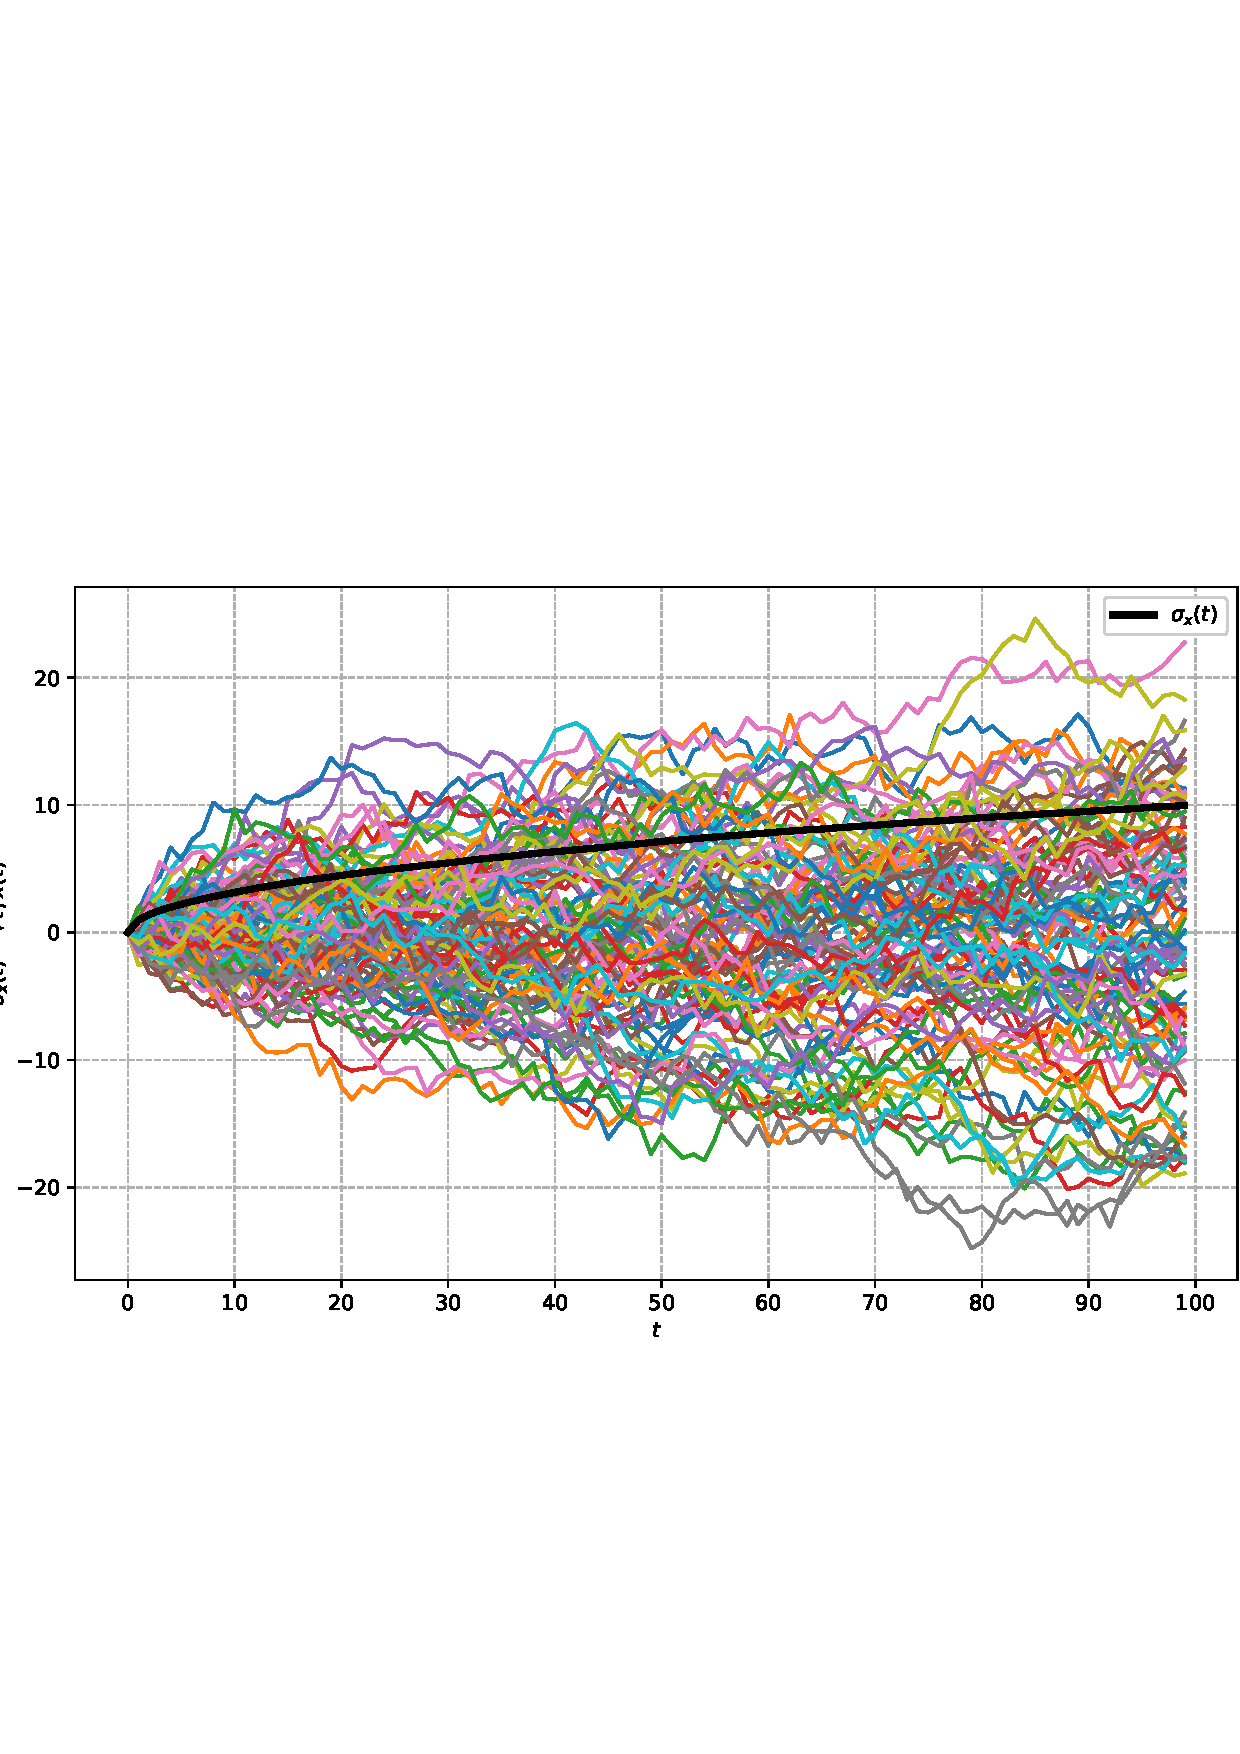
\includegraphics[width=0.9\textwidth]{images/normal_rw.pdf}
  \caption{چند نمونه مستقل از فرایند ولگشت تصادفی که قدم‌هایی با توزیع گاوسی برمی‌دارد.}
\end{figure}
\FloatBarrier

\section{فرایندهای مارکوف}
\label{sec:markov}

همان‌طور که گفته شد در صورتی که توزیع احتمال توأم $n$ نقطه‌ای  یک فرایند تصادفی را داشته باشیم، همه اطلاعات ممکن برای یک فرایند تصادفی تا زمان $t_n$ را می‌توانیم از روی توزیع احتمال توأم به دست آوریم. در حالتی که توزیع احتمال فرایند تصادفی در هر زمان به زمان‌های قبل از خودش وابستگی نداشته باشد و مستقل رفتار کند، توزیع احتمال توأم $n$ نقطه‌ای از ضرب احتمال متغیر تصادفی در زمان‌های مختلف به دست می‌آید. یعنی:
\begin{equation}
  p(x_n,t_n; x_{n-1},t_{n-1} \dotsc ;x_{0},t_0)  = p(x_{n}, t_{n}) p(x_{n-1}, t_{n-1}) \dotsc p(x_0,t_0)
  \label{n_point_joint}
\end{equation}
به فرایندی که از رابطه بالا پیروی کند فرایند تصادفی مستقل گفته می‌شود. کاربرد این‌گونه فرایندها بسیار محدود است، بنابراین به مدل‌های تصادفی بهتری نیاز داریم.
یکی از پرکاربرد ترین نوع فرایندهای تصادفی، فرایندهای مارکوف هستند. ایده اصلی فرایندهای مارکوف این است که حالت آینده یک فرایند تصادفی فقط به حالت کنونی فرایند وابسته است و از گام‌های زمانی قبل مستقل است پس می‌توان نتیجه گرفت که  توزیع احتمال این نوع فرایندها در هر زمان فقط به زمان قبلی وابسته است، یعنی:
\begin{equation}
  p(x_n,t_n \mid x_{n-1},t_{n-1} \dotsc ;x_{0},t_0) = p(x_n,t_n \mid x_{n-1},t_{n-1})
  \label{markov_def}
\end{equation}
 که رابطه بالا به ازای همه $n$ها برقرار است. بنابراین می‌توان توزیع احتمال توأم $n$ نقطه‌ای را به صورت زیر به دست آورد 
 \begin{equation}
  \begin{array}{l}
    p(x_n,t_n; x_{n-1},t_{n-1} \dotsc ;x_{0},t_0)\\ \qquad = p(x_{n},t_n\mid x_{n-1},t_{n-1}) \dotsc p(x_{2},t_{2} \mid x_{1},t_{1}) p(x_{1},t_{1} \mid x_{0},t_{0}) p(x_0,t_0)
    \label{markov}
  \end{array}
\end{equation}
به احتمال‌های شرطی دو تایی در فرایندهای مارکوف، احتمال انتقال هم گفته می‌شود در شرایطی که این احتمال به زمان وابستگی نداشته باشد و فقط به اختلاف زمانی وابسته باشد به این فرایند، فرایند همگن\LTRfootnote{Homogenous Markov chain} گفته می‌شود. 
به عنوان مثالی از فرایندهای مارکوف همگن فرض کنید اگر امروز هوا آفتابی یا بارانی باشد بر روی شرایط آب و هوای فردا تأثیر گذار باشد و مهم نباشد که در چو موقعی از سال قرار داریم. شکل زیر نمایشی از ماتریس انتقال برای این مثال است.
\begin{figure}[H]
  \centering
  \includegraphics[width=0.4\textwidth]{images/weather_chain.pdf}
  \caption{زنجیره مارکوف} \label{fig:weather_chain}
  \par\medskip
\captionsetup{justification=centering}
\end{figure}
\FloatBarrier

اغلب به فرایندهای مارکوف با زمان گسسته و فضای نمونه شمارا، زنجیره مارکوف هم گفته می‌شود. در جدول زیر انواع فرایندهای مارکوف در شرایط مختلف آورده شده است، هرچند بر روی این تقسیم‌بندی و برخی اصطلاحات توافقی وجود ندارد. اما استفاده از نام زنجیره مارکوف برای فرایندهای با زمان و فضای نمونه گسسته رایج است.\cite{gagniuc_markov_2017}
\begin{table}[htb]
  \centering
  \caption{تقسیم‌بندی فرایندهای مارکوف}
  \begin{tabular}{|C{4cm}|C{4cm}|C{4cm}|}
    \hline
    \cellcolor[HTML]{C0C0C0} & فضای نمونه شمارا                               & فضای نمونه پیوسته                             \\ \hline
    زمان گسسته               & زنجیره مارکوف                                  & زنجیره مارکوف روی فضای نمونه قابل اندازه‌گیری \\ \hline
    زمان پیوسته              & فرایند مارکوف زمان‌پیوسته یا فرایند پرش مارکوف & دیگر فرایندهای تصادفی با خاصیت مارکوف         \\ \hline
    \end{tabular}
\end{table}
\FloatBarrier

از این پس تمام روابط برای فرایند مارکوف با فضای نمونه و زمان پیوسته نوشته خواهند شد اما در ادامه به بررسی چند ویژگی مهم می‌پردازیم که بیشتر برای زنجیره‌های مارکوف استفاده می‌شوند.

\subsection{حد مانای فرایندهای مارکوف}

برخی فرایندهای مارکوف پس از گذشت زمان کافی به حالتی مانا می‌رسند.
در این بخش به بررسی روشی برای یافتن حالت مانا فرایندهای مارکوف می‌پردازیم که بیشتر برای زنجیره‌های مارکوف کاربردی است.
با توجه به رابطه \ref{j_prob_cond} می‌توانیم بنویسیم.
$$
  p(x_{i+1},t_{i+1};x_{i}, t_{i}) = p(x_{i+1},t_{i+1} \mid x_{i}, t_{i}) p(x_{i},t_{i})
$$
که $x_i$ و $x_{i+1}$، متغیر تصادفی $x$ را در دو زمان متوالی $t_i$ و $t_{i+1}$ نشان می‌دهد. با استفاده از رابطه \ref{marginalization} و جمع زدن بر روی $x_i$ می‌توانیم توزیع احتمال $x_{i+1}$ را در زمان $t_{i+1}$ به دست آوریم.
\begin{equation}
  p(x_{i+1},t_{i+1}) = \int_{-\infty}^{+\infty} p(x_{i+1},t_{i+1} \mid x_{i}, t_{i}) p(x_{i},t_{i}) d x_{i}
  \label{transition_multip}
\end{equation}
رابطه بالا در‌واقع نشان دهنده ضرب ماتریس انتقال $\mathbf{p_{i+1,i}}$ در بردار توزیع احتمال $\mathbf{p_i}$ است.
$$
  \mathbf{p_{i+1}} = \mathbf{p_{i+1,i}} \times \mathbf{p_i}
$$
که حروف پررنگ نشان‌دهنده شکل ماتریسی و برداری است.
اگر $\mathbf{p_{i+2,i+1}}$ را در دو طرف رابطه بالا ضرب کنیم.
$$
  \mathbf{p_{i+2}} = \mathbf{p_{i+2,i+1}} \times \mathbf{p_{i+1,i}} \times \mathbf{p_i}
$$
در حالتی که فرایند همگن باشد یعنی $p(x_{i+2}, t_{i+2} \mid x_{i+1},t_{i+1})=p(x_{i+1},t_{i+1} \mid x_{i}, t_{i})$ باشد و ماتریس انتقال را نیز با $\mathbf{W}=\mathbf{p_{i+2,i+1}} = \mathbf{p_{i+1,i}}$ نشان دهیم خواهیم داشت.
$$
  \mathbf{p_{i+2}} = \mathbf{W}^{2} \times \mathbf{p_{i}}
$$
رابطه بالا یکی از نتیاج مهم برای فرایندهای مارکوف همگن است، اگر این کار را ادامه دهیم می‌توانیم احتمال انتقال برای $n$ گام زمانی را برای یک فرایند مارکوف همگن به دست آوریم. که به شکل زیر به دست می‌آید.
\begin{equation}
    \mathbf{p_{n}} = \mathbf{W}^{n} \times \mathbf{p_{0}}
    \label{nstep_transition}
\end{equation}
با فرض اینکه حالت مانای فرایند $x$ وجود دارد و $p_{s}(x)$ نشان دهنده توزیع احتمال $x$ در زمان $t_s$ باشد یعنی زمانی که فرایند به حالت مانای خود رسیده است، اگر ماتریس انتقال را در این احتمال ضرب کنیم، توزیع به دست آمده باید برابر $p_{s}(x)$ باشد.\cite{bremaud_markov_1999}
$$
\mathbf{p_{s}(x)} = \mathbf{W}^{n} \times \mathbf{p_{s}(x)}
$$
رابطه بالا در فیزیک به معادله ویژه برداری معروف است، با حل این معادله می‌توان $p_{s}(x)$ را به دست آورد.

\subsection{معادله چَپمَن-کولموگروف}

با توجه به رابطه \ref{marginalization} دیدیم که توزیع‌های احتمال توأم چگونه به هم مرتبط هستند اگر بخواهیم احتمال توأم دونقطه‌ای را از احتمال توأم سه نقطه‌ای به دست آوریم داریم:
$$
  p\left(x_{3}, t_{3} ; x_{1}, t_{1}\right)=\int_{-\infty}^{+\infty} p\left(x_{3}, t_{3}; x_{2}, t_{2}; x_{1}, t_{1}\right) d x_{2}
$$
 اگر $x$ یک فرایند مارکوف باشد بنابراین $p(x_{3}, t_{3} ; x_{2}, t_{2}; x_{1}, t_{1}) = p(x_{3}, t_{3} \mid x_{2}, t_{2}) p(x_{2}, t_{2} \mid x_{1}, t_{1}) p(x_{1}, t_{1})$ با جایگذاری در رابطه بالا داریم:
 \begin{equation}
  p\left(x_{3}, t_{3}; x_{1}, t_1\right)=\int_{-\infty}^{+\infty} p\left(x_{3}, t_3 \mid x_{2}, t_2\right) p\left(x_{2}, t_2 \mid x_{1}, t_1\right) p\left(x_{1}, t_1\right) d x_{2}
  \label{ck_equation}
\end{equation}
معادله بالا به معادله چپمن-کولموگروف\LTRfootnote{Chapman-Kolmogorov equation} معروف است و باید توجه شود که معادله بالا برای سه زمان متوالی $t_1$، $t_2$ و $t_3$ نوشته شده است. اگر دو طرف تساوی را به $p(x_{1}, t_1)$ تقسیم کنیم با توجه به رابطه احتمال شرطی و توأم \ref{cond_prob_j} به شکل دیگری از معادله چپمن-کولموگروف می‌رسیم.
\begin{equation}
  p\left(x_{3}, t_3 \mid x_{1}, t_1\right)=\int_{-\infty}^{+\infty} p\left(x_{3}, t_3 \mid x_{2}, t_2\right) p\left(x_{2}, t_2 \mid x_{1}, t_1\right) d x_{2}
  \label{ck_equation_cond}
\end{equation}
معادله چپمن-کولموگروف برای همه‌ی فرایندهای مارکوف برقرار است، اما هر فرایندی که معادله چپمن-کولموگروف برای آن برقرار باشد لزوماً مارکوف نیست. به عبارت دیگر برقرار بودن معادله چپمن-کولموگروف شرط لازم برای یک فرایند مارکوف است.

\subsection{فرایند وینر}

یک مثال پرکاربرد از فرایندهای مارکوف، فرایند وینر\LTRfootnote{Wiener process} است. فرایند وینر از بسیاری جهات مشابه یک ولگشت تصادفی با قدم‌های گاوسی است، با این تفاوت که توزیع قدم‌ در هر زمان به قدم قبلی وابسته است. احتمال انتقال فرایند وینر به شکل زیر است:
\begin{equation}
  p_{2}\left(x, t \mid x^{\prime}, t^{\prime}\right)=\frac{1}{\sqrt{2 \pi \tau}} e^{-\left(x-x^{\prime}\right)^{2} / 2 \tau}
\end{equation}
که $\tau = t - t^\prime$ است، بنابراین فرایند وینر یک فرایند مارکوف همگن است که احتمال انتقال آن فقط به $\tau$ وابسته است. توزیع احتمال این فرایند در هر زمان به شکل زیر است.
\begin{equation}
  p_{1}(x, t)=\frac{1}{\sqrt{2 \pi t}} e^{-x^{2} / 2 t}
  \end{equation}
فرایند وینر را در فیزیک می‌توان به عنوان فرایند پخش گرما یا حرکت براونی ذرات تعبیر کرد. نکته مهم در مورد فرایند وینر این است که این فرایند حد مانا ندارد.\cite{risken_fokker-planck_1984}

\subsection{معادله مادر}

برای فهمیدن رفتار یک فرایند مارکوف معادله چپمن-کولموگروف کمک زیادی نخواهد کرد اما می‌توان از معادله چپمن-کولموگروف به معادله‌ای سودمند به نام معادله مادر\LTRfootnote{Master equation} رسید. 
معادله مادر یک معادله دیفرانسیلی برای احتمال انتقال است که تغییرات احتمال انتقال بر حسب زمان را به دست می‌دهد. برای به دست آوردن این معادله باید رفتار احتمال انتقال را در اختلاف زمان‌های کوتاه یعنی $\Delta t \rightarrow 0$ مشخص کنیم. در معادله \ref{ck_equation_cond} به ازای $t_2 = t_1 = t$ به نتیجه بدیهی زیر می‌رسیم.
$$
\begin{array}{l}
  p\left(x_{3} , t_{3} \mid x_{1} , t_{1}\right) = \int_{-\infty}^{+\infty} p\left(x_{3} , t_{3} \mid x_{2} , t \right) p\left(x_{2} , t \mid x_{1} , t \right) d x_{2} \\
  \qquad \Rightarrow p\left(x_{2} , t \mid x_{1} , t \right) = \delta\left( x_2 - x_1 \right) 
\end{array}
$$
که تابع دلتا به دست آمده در‌واقع مرتبه صفرم از رفتار $p(x^\prime,t^\prime \mid x,t)$ در زمان‌های کوتاه است. با در نظر داشتن این نکته می‌توان رابطه زیر را برای رفتار احتمال انتقال در زمان‌های کوتاه به دست آورد.
\begin{equation}
  p\left(x_{2}, t+\Delta t \mid x_{1}, t\right)=\delta\left(x_{2}-x_{1}\right)\left[1-a^{(0)}\left(x_{1}, t\right) \Delta t\right]+w_{t}\left(x_{2} \mid x_{1}\right) \Delta t+O\left[(\Delta t)^{2}\right]
  \label{transition_zero_order}
\end{equation}
در رابطه بالا $w_{t}(x_2 \mid x_1)$ را به عنوان احتمال انتقال از $x_{1}$ به $x_{2}$ بر واحد زمان $t$ تعبیر می‌کنیم. بنابراین ضریب $1-a^{(0)}\left(x_{1}, t\right) \Delta t$ را باید احتمال اینکه هیچ انتقالی در مدت زمان $\Delta t$ صورت نگیرد تعبیر کرد یعنی احتمال اینکه در این مدت زمان  $x$ ثابت باشد. از نرمال بودن احتمال انتقال $p(x_2,t_2 \mid x_1,t_1)$ می‌توانیم بنویسیم.
$$
1=\int \mathrm{d} x_{2} P\left(x_{2}, t+\Delta t \mid x_{1}, t\right) \simeq 1-a^{(0)}\left(x_{1}, t\right) \Delta t+\int \mathrm{d} x_{2} w_{t}\left(x_{2} \mid x_{1}\right) \Delta t
$$
بنابراین داریم
\begin{equation}
  a^{(0)}\left(x_{1}, t\right)=\int \mathrm{d} x_{2} w_{t}\left(x_{2}  \mid  x_{1}\right)
  \label{cond_moment_zero}
\end{equation}
از رابطه بالا می‌بینیم که $a^{(0)}\left(x_{1}, t\right) \Delta t$ احتمال کل انتقال از $x_{1}$ در بازه $(t,t+\Delta t)$را نشان می‌دهد بنابراین $1 - a^{(0)}\left(x_{1}, t\right) \Delta t$ احتمال این است که هیچ انتقالی در این بازه اتفاق نیفتد.

حالا می‌توانیم با استفاده از معادله چپمن-کولموگروف \ref{ck_equation_cond} معادله دیفرانسیلی برای احتمال انتقال به دست آوریم. با جایگذاری رابطه \ref{transition_zero_order} در معادله چپمن-کولموگروف \ref{ck_equation_cond} به ازای $t_{3} = t_{2} + \Delta t$ داریم:

$$
\begin{aligned} p\left(x_{3}, t_{2}+\Delta t  \mid  x_{1}, t_{1}\right)=& \int \mathrm{d} x_{2} \overbrace{p\left(x_{3}, t_{2}+\Delta t \mid x_{2}, t_{2}\right)}^{\hidewidth \delta\left(x_{3}-x_{2}\right)\left[1-a^{(0)}\left(x_{2}, t_{2}\right) \Delta t\right]+w_{t_{2}}\left(x_{3}  \mid  x_{2}\right) \Delta t \hidewidth } p\left( x_{2}, t_{2} \mid x_{1} , t_{1} \right)\\ \simeq &\left[1-a^{(0)}\left(x_{3}, t_{2}\right) \Delta t\right] p\left(x_{3}, t_{2}  \mid  x_{1}, t_{1}\right) \\ &+\Delta t \int \mathrm{d} x_{2} w_{t_{2}}\left(x_{3}  \mid  x_{2}\right) p\left(x_{2}, t_{2}  \mid  x_{1}, t_{1}\right) \end{aligned}
$$
 سپس  $a^{(0)}\left(x_{3}, t_{2}\right)$ را با استفاده از \ref{cond_moment_zero} بر حسب $w_{t_{2}}(x_{2} \mid x_{3})$ می‌نویسیم. بنابراین رابطه بالا را به شکل زیر می‌نویسیم.
$$
\begin{aligned} \frac{1}{\Delta t}\left[p\left(x_{3}, t_{2}\right.\right.&\left.\left.+\Delta t \mid x_{1}, t_{1}\right)-p\left(x_{3}, t_{2} \mid x_{1}, t_{1}\right)\right] \\ & \simeq \int \mathrm{d} x_{2}\left[w_{t_{2}}\left(x_{3} \mid x_{2}\right) p\left(x_{2}, t_{2} \mid x_{1}, t_{1}\right)-w_{t_{2}}\left(x_{2} \mid x_{3}\right) p\left(x_{3}, t_{2} \mid x_{1}, t_{1}\right)\right] \end{aligned}
$$
نشان گذاری  را با تبدیل $x_{1}$ و $t_{1}$ به $x_{0}$ و $t_{0}$، $x_{2}$ و $t_{2}$ را به $x^\prime$ و $t^\prime$   و در نهایت $x_{3}$ را به $x$ تغییر می‌دهیم. بنابراین در حد $\Delta t \rightarrow 0$ می‌توانیم معادله مادر را به شکل زیر به دست آوریم.
\begin{equation}
  \frac{\partial}{\partial t} p\left(x, t \mid x_{0}, t_{0}\right)=\int \mathrm{d} x^{\prime}\left[w_{t}\left(x | x^{\prime}\right) p\left(x^{\prime}, t \mid x_{0}, t_{0}\right)-w_{t}\left(x^{\prime} \mid x\right) p\left(x, t \mid x_{0}, t_{0}\right)\right]
  \label{master_equation_transition}
\end{equation}
که یک معادله انتگرال – دیفرانسیل است. معادلات انتگرال – دیفرانسیل معادلاتی هستند که شامل انتگرال و مشتق یک تابع هستند.

معادله مادر یک شکل دیفرانسیلی از معادله چپمن-کولموگروف است. بنابراین نمی‌توان با آن توزیع احتمال $p\left( x, t \right)$ را حساب کرد و برای محاسبه احتمال انتقال $p\left( x,t \mid x_{0},t_{0} \right)$ کاربرد دارد. اما می‌توان نشان داد که با در نظر گرفتن شرایط اولیه می‌توان معادله‌ای برای توزیع احتمال با استفاده از معادله مادر به شکل زیر به دست آورد.\cite{2007cond.mat..1242G}
\begin{equation}
  \frac{\partial p(x, t)}{\partial t}=\int \mathrm{d} x^{\prime}\left[w\left(x \mid x^{\prime}\right) p\left(x^{\prime}, t\right)-w\left(x^{\prime} \mid x\right) p(x, t)\right]
  \label{master_equation}
\end{equation}
از شکل معادله مادر می‌بینیم که این معادله در‌واقع یک معادله توازن برای احتمال حالت‌های (مقادیر) ممکن $x$ است.

\subsection{بسط کرامرز-مویال و معادله فوکر-پلانک}

بسط کرامرز-مویال\LTRfootnote{Kramers–Moyal expansion} معادله مادر را از یک معادله انتگرال – دیفرانسیل به یک معادله دیفرانسیل با مرتبه بی‌نهایت تبدیل می‌کند. بنابراین استفاده از این بسط از معادله مادر آسان‌تر نیست اما تحت شرایطی ممکن است که بتوان با تعداد محدودی از جملات بسط معادله را حل کرد.\cite{kramers_brownian_1940}

در ابتدا با یک تغییر متغیر احتمال انتقال $w$ را به تابعی بر حسب $r$ که $r=x^\prime - x$ تبدیل می‌کنیم. یعنی احتمال انتقال تابعی است از میزان جابه‌جایی $r$ و نقطه شروع $x^\prime$، بنابراین داریم:
\begin{equation}
  w\left( x \mid x^{\prime} \right) = w\left(x^{\prime} ; r\right), \quad r=x-x^{\prime}
  \label{transition_cfv}
\end{equation}
بنابراین معادله مادر \ref{master_equation} را می‌توان به شکل زیر نوشت.
\begin{equation}
  \frac{\partial p(x, t)}{\partial t}=\int w(x-r ; r) p(x-r, t) \mathrm{d} r - p(x, t) \int w(x ;-r) \mathrm{d} r
  \label{master_eq_1}
\end{equation}
 که تغییر علامت مربوط به تغییر متغیر $x^\prime \rightarrow r = x - x^\prime$ در کران‌های انتگرال به این شکل تأثیر گذاشته است که
$$
  \int_{-\infty}^{\infty} \mathrm{d} x^{\prime} f\left(x^{\prime}\right)=-\int_{x+\infty}^{x-\infty} \mathrm{d} r f(x-r)=-\int_{\infty}^{-\infty} \mathrm{d} r f(x-r)=\int_{-\infty}^{\infty} \mathrm{d} r f(x-r)
$$
با فرض اینکه تغییرات $x$ به شکل پرش‌های کوچک اتفاق می‌افتد بنابراین $w(x^\prime;r)$ یک تابع تیز از $r$ است اما تغییرات آن با $x^\prime$ به اندازه کافی آرام است. فرض دیگری که می‌کنیم این است که $p(x,t)$ نیز به آرامی با $x$ تغییر می‌کند. حال می‌توانیم تغییر $x$ به $x-r$ را با بسط تیلور بررسی کنیم بنابراین جمله اول سمت راست رابطه \ref{master_eq_1} را بسط تیلور می‌دهیم.
$$
\begin{aligned} \frac{\partial p(x, t)}{\partial t}=& \int w(x ; r) p(x, t) \mathrm{d} r+\sum_{m=1}^{\infty} \frac{(-1)^{m}}{m !} \int r^{m} \frac{\partial^{m}}{\partial x^{m}}[w(x ; r) p(x, t)] \mathrm{d} r  \\ &-p(x, t) \int w(x ;-r) \mathrm{d} r \\=& \sum_{m=1}^{\infty} \frac{(-1)^{m}}{m !} \frac{\partial^{m}}{\partial x^{m}}\left\{\left[\int r^{m} w(x ; r) \mathrm{d} r \right] p(x, t)\right\} \end{aligned}
$$
که جمله اول و سوم در رابطه بالا با یکدیگر ساده شده‌اند بنابراین داریم.
در انتها ضرایب بسط به شکل زیر تعریف می‌کنیم.
\begin{equation}
  a^{(m)}(x, t)=\int r^{m} w(x ; r) \mathrm{d} r
  \label{jump_moments}
\end{equation}
بنابراین بسط کرامرز-مویال معادله مادر به شکل زیر به دست می‌آید. 
\begin{equation}
  \frac{\partial p(x, t)}{\partial t}=\sum_{m=1}^{\infty} \frac{(-1)^{m}}{m !} \frac{\partial^{m}}{\partial x^{m}}\left[a^{(m)}(x, t) p(x, t)\right]
  \label{kramers_moyal}
\end{equation}
بسط کرامرز-مویال هیچ تفاوتی با معادله مادر ندارد پس استفاده از این بسط به اندازه معادله مادر مشکل است. اما همان‌طور که گفته شد ممکن است تحت شرایطی بتوان از جملات مرتبه بالا بسط کرامز مویال صرف نظر کرد. مثلاً در شرایطی که به ازای $m > 2$ ضرایب $a^{m}(x,t)$ خیلی کوچک باشند و بتوان از آن‌ها صرف نظر کرد، بسط کرامرز-مویال به شکل زیر تبدیل می‌شود.
\begin{equation}
  \frac{\partial p(x, t)}{\partial t}=-\frac{\partial}{\partial x}\left[a^{(1)}(x, t) p(x, t)\right]+\frac{1}{2} \frac{\partial^{2}}{\partial x^{2}}\left[a^{(2)}(x, t) p(x, t)\right]
  \label{fokker_plank}
\end{equation}
به معادله بالا، معادله فوکر-پلانک\LTRfootnote{Fokker–Planck equation} گفته می‌شود. به جمله اول این معادله جمله رانش و به جمله دوم آن جمله پخش گفته می‌شود، همچنین به ضرایب $a^{1}(x,t)$ و $a^{2}(x,t)$ ضریب رانش و ضریب پخش گفته می‌شود. یادآوری این نکته لازم است که معادله فوکر-پلانک به عنوان حالت خاصی از بسط کرامرز-مویال از معادله مادر به دست می‌آید، بنابراین این معادله نیز رفتار احتمال انتقال را در زمان نشان می‌دهد اما همان‌طور که گفته شد با در نظر گرفتن شرایط اولیه می‌توان رفتار توزیع احتمال را همان‌طور که در \ref{fokker_plank} نوشته شده است نیز به دست آورد.\cite{moyal_stochastic_1949}

\subsection{ممان‌های شرطی}

احتمال انتقال بر واحد زمان $w(x^\prime \mid x)$ در تعریف ممان‌های شرطی \ref{jump_moments} استفاده شده است. بنابراین مجبوریم برای محاسبه $a^{m}(x.t)$ از رابطه \ref{transition_zero_order} که رابطه بین $w(x^\prime \mid x)$ و احتمال انتقال برای اختلاف زمان‌های کوچک است، استفاده کنیم.
در رابطه \ref{transition_cfv} دیدیم که $w(x^\prime ; r) = w(x \mid x^\prime)$ و $x = x^\prime + r$ بر همین اساس می‌توانیم بنویسیم:
$$
w(x ; r)=w\left(x^{\prime} \mid x\right), \quad x^{\prime}=x+r
$$
با جایگذاری این عبارت در معادله \ref{jump_moments} می‌توان نوشت.
\begin{equation}
  a^{(m)}(x, t)=\int \mathrm{d} x^{\prime}\left(x^{\prime}-x\right)^{m} w\left(x^{\prime} \mid x\right)
\end{equation}
به منظور اینکه رابطه‌ای برای ضرایب به دست بیاوریم کمیت زیر را معرفی می‌کنیم.
\begin{equation}
  \mathcal{A}^{(m)}(x ; \tau, t)=\int \mathrm{d} x^{\prime}\left(x^{\prime}-x\right)^{m} p\left(x^{\prime}, t+\tau \mid x, t\right)
\end{equation}
که در‌واقع میانگین $[X(t + \tau) - X(t)]^{m}$ به ازای $X(t) = x$ است و به آن ممان شرطی می‌گویند. سپس با استفاده از احتمال انتقال برای زمان‌های کوتاه \ref{transition_zero_order} می‌توانیم بنویسیم

$$
\begin{aligned} \mathcal{A}^{(m)}(x ; \tau, t) &=\int \mathrm{d} x^{\prime}\left(x^{\prime}-x\right)^{m}\left\{\delta\left(x^{\prime}-x\right)\left[1-a^{(0)}(x, t) \tau\right]+w\left(x^{\prime} \mid x\right) \tau+\mathcal{O}\left(\tau^{2}\right)\right\} \\ &=\tau \int \mathrm{d} x^{\prime}\left(x^{\prime}-x\right)^{m} w\left(x^{\prime} \mid x\right)+\mathcal{O}\left(\tau^{2}\right) \\ &=a^{(m)}(x, t) \tau+\mathcal{O}\left(\tau^{2}\right), \quad(m \geq 1) \end{aligned}
$$
که اولین جمله انتگرال به دلیل وجود تابع دلتای دیراک از بین می‌رود. بنابراین می‌توان ضرایب بسط را از مشتق ممان‌های شرطی به شکل زیر به دست آورد
\begin{equation}
a^{(m)}(x, t)=\left.\frac{\partial}{\partial \tau} \mathcal{A}^{(m)}(x ; \tau, t)\right|_{\tau=0}
\label{cond_moment_km}
\end{equation}
در انتها با نوشتن $\mathcal{A}$ به شکل زیر:
$$
\mathcal{A}^{(m)}(x ; \Delta t, t)=\int \mathrm{d} x^{\prime}\left(x^{\prime}-x\right)^{m} p\left(x^{\prime}, t+\Delta t  \mid  x, t\right)=\left.\left\langle[X(t+\Delta t)-X(t)]^{m}\right\rangle\right|_{X(t)=x}
$$
می‌توانیم ضرایب بسط را با استفاده از رابطه زیر به دست آوریم.
\begin{equation}
a^{(m)}(x, t)=\left.\lim _{\Delta t \rightarrow 0} \frac{1}{\Delta t}\left\langle[X(t+\Delta t)-X(t)]^{m}\right\rangle\right|_{X(t)=x}
\label{exp_coef}
\end{equation}

\subsection{قضیه پاوولا}
همان‌طور که دیدیم بسط کرامرز-مویال دارای تعداد نامتناهی جمله است که در حالت کلی حل این بسط را نسبت به معادله مادر ساده‌تر نمی‌کند، اما اگر بتوان تعدادی از جملات را نگه داشت و از بقیه آن‌ها صرف نظر کرد حل بسط کرامرز-مویال بسیار ساده‌تر از معادله مادر خواهد بود. برای اینکه بتوانیم از این جملات صرف نظر کنیم، ممان‌های متعلق به این جملات باید صفر باشند. اما بررسی کردن تعداد نامتناهی ممان به اندازه حل بسط کرامرز-مویال کار دشواری است. با روشی که قضیه پاوولا\LTRfootnote{Pawula theorem} معرفی می‌کند می‌توانیم از صفر بودن ممان‌ها، بدون بررسی تک‌تک آن‌ها مطمئن شویم. 
بدین منظور باید از حالت کلی نامساوی شوارتز استفاده کنیم که به شکل زیر است.
\begin{equation}
  [f(x) g(x) P(x) \mathrm{d} x]^{2} \leq \int f^{2}(x) P(x) \mathrm{d} x \int g^{2}(x) P(x) \mathrm{d} x
\end{equation}
در نامساوی بالا $P(x)$ یک تابع مثبت است و توابع $f(x)$ و $g(x)$ توابع دلخواهی هستند.
$$
\begin{array}{l}{f(x)=\left(x-x^{\prime}\right)^{n} ; \quad g(x)=\left(x-x^{\prime}\right)^{n+m}} \\ {P(x)=P\left(x, t+\tau | x^{\prime}, t^{\prime}\right)}\end{array}
$$
به ازای توابع به شکل بالا نامساوی شوارتز به عبارت زیر که بین ممان‌های شرطی است تبدیل می‌شود.\cite{risken_fokker-planck_1984}
\begin{equation}
  \mathcal{A}_{2 n+m}^{2} \leq \mathcal{A}_{2 n} \cdot \mathcal{A}_{2 n+2 m}
  \label{inequality_moments}
\end{equation}
برای $n=0$ داریم $\mathcal{A}_{m} \leq \mathcal{A}_{2m}$  که این رابطه به وضوح برای $m = 0$ برقرار است. از این رابطه هیچ محدودیتی برای ضرایب بسط $a^{(m)}(x, t)$ به دست نمی‌آید. به ازای $m = 0$ رابطه \ref{inequality_moments} به $\mathcal{A}^{2}_{2n} \leq \mathcal{A}^{2}_{2n}$ تبدیل می‌شود که به ازای همه $n$ها برقرار است. بنابراین ناچاریم که رابطه \ref{inequality_moments} را به ازای $n \geq 1$ و $m \geq 1$ بررسی کنیم. از دو طرف رابطه \ref{inequality_moments} نسبت به $\tau$ مشتق می‌گیریم و به ازای $\tau = 0$ این رابطه به رابطه‌ای مشابه برای ضرایب بسط $a^{(m)}(x, t)$ تبدیل می‌شود.
\begin{equation}
  [a^{(2 n+m)}]^{2} \leq a^{(2 n)} \cdot a^{(2 n+2 m)}
  \label{inequality_coeff}
\end{equation}
اگر $a^{(2 n)} = 0$ صفر باشد بنابراین $a^{(2 n + m)}$ هم حتماً صفر است، به عبارت دیگر:
\begin{equation}
  a^{(2 n)}=0 \Rightarrow a^{(2 n+1)}=a^{(2 n+2)}=\ldots=0 \quad(n \geq 1)
  \label{pawula1}
\end{equation}
علاوه بر این اگر $a^{(2 n + 2 m)}$ صفر باشد، $a^{(2 n + m)}$ هم حتماً صفر است، به عبارت دیگر اگر $r = n + m$ در نظر بگیریم، داریم:
\begin{equation}
\begin{array}{l}{a^{(2 r)}=0 \Rightarrow a^{(r+n)}=0 \quad(n=1, \ldots, r-1)} \\ \qquad \Rightarrow {a^{(2 r-1)}=a^{(2 r-2)}=\ldots=a^{(r+1)}=0 \quad(r \geq 2)}\end{array}
  \label{pawula2}
\end{equation}
با استفاده از \ref{pawula1} و \ref{pawula2} می‌توان به این نتیجه رسید که به ازای $r \geq 1$ اگر داشته باشیم $a^{(2 r)}=0$ تمام ضرایب $a^{(n)}$ به ازای $n \geq 3$ نیز صفر خواهند شد. به عبارت دیگر:
\begin{equation}
  a^{(2 n)}=0 \Rightarrow a^{(3)}=a^{(4)}=\ldots=0 \quad(n \geq 1)
  \label{pwula}
\end{equation}
رابطه بالا چیزی است که به آن قضیه پاوولا گفته می‌شود و اگر شرط بالا برقرار باشد بسط کرامرز-مویال به معادله فوکر-پلانک تبدیل می‌شود.\cite{pawula_generalizations_1967}

\section{معادله لانژوین}

تا اینجا فرایندهای تصادفی را با استفاده از توزیع احتمال آن‌ها بررسی کرده‌ایم. در این بخش روش متفاوتی را در پیش می‌گیریم و به جای بررسی تحول زمانی توزیع احتمال، به شکل مستقیم تحول زمانی متغیر تصادفی را بررسی می‌کنیم. رابطه زیر شکل کلی معادله لانژوین\LTRfootnote{Langevin equation} است.\cite{lemons_paul_1997}

\begin{equation}
\frac{\mathrm{d} x}{\mathrm{d} t}=A(x, t)+B(x, t) \zeta(t)
\label{langevin}
\end{equation}
در رابطه بالا $\zeta (t)$ یک فرایند تصادفی دلخواه است که به آن نیروی تصادفی هم گفته می‌شود. انتخاب $\zeta (t)$ مناسب باعث می‌شود که $x(t)$ یک فرایند مارکوف باشد. اگر $\zeta (t)$ توزیع گاوسی با آمار زیر باشد، متغیر تصادفی $x(t)$ خاصیت مارکوف خواهد داشت.
\begin{equation}
\begin{aligned}\langle\zeta(t)\rangle &= 0 \\\left\langle\zeta\left(t_{1}\right) \zeta\left(t_{2}\right)\right\rangle &= 2 D \delta\left(t_{1}-t_{2}\right) \end{aligned}
  \label{noise_term_properties}
\end{equation}
از آنجایی که معادله \ref{langevin} یک معادله دیفرانسیل مرتبه اول است، هر نمونه از $\zeta(t)$ با مشخص بودن شرایط اولیه $x(t_{0})$، $x(t)$ به صورت یکتا مشخص می‌شود. علاوه بر این ، مقادیر جمله دوم در زمان‌های متفاوت مستقل از هم هستند، به دلیل اینکه همبستگی $\zeta(t)$ به شکل تابع دلتای دیراک است. بنابراین مقادیر $\zeta(t)$ در زمان‌های قبل مثلاً $t^\prime < t_{0}$ نمی‌توانند تأثیری بر احتمال‌های شرطی در زمان‌‌های $t > t_{0}$ بگذارند. با توجه به شرایط گفته شده می‌توان نتیجه گرفت که جواب معادله لانژوین \ref{langevin} دارای خاصیت مارکوف است. 

جمله $A(x,t)$ و $B(x,t)\zeta(t)$ را اغلب با نام جمله رانش و جمله پخش می‌شناسند. به دلیل وجود $\zeta(t)$ معادله \ref{langevin} یک معادله دیفرانسیل تصادفی است که به معنی وجود جملات تصادفی در معادله است که باعث به وجود آمدن خواص تصادفی در $x(t)$ می‌شود. حل یک معادله لانژوین به معنی یافتن خواص آماری فرایند $x(t)$ است.

\subsection{ضرایب بسط کرامرز-مویال و معادله لانژوین}

از آنجایی که جواب معادله لانژوین یک فرایند مارکوف است، بنابراین باید از یک معادله مادر پیروی کند که می‌توانیم آن را به شکل بسط کرامرز-مویال \ref{kramers_moyal} بنویسیم. حال می‌خواهیم ضرایب بسط \ref{exp_coef} را برای یک معادله لانژوین به دست آوریم. برای این کار معادله \ref{langevin} را به یک معادله انتگرالی تبدیل می‌کنیم.
\begin{equation}
  x(t+\Delta t)-x=\int_{t}^{t+\Delta t} \mathrm{d} t_{1} A\left[x\left(t_{1}\right), t_{1}\right]+\int_{t}^{t+\Delta t} \mathrm{d} t_{1} B\left[x\left(t_{1}\right), t_{1}\right] \zeta\left(t_{1}\right)
  \label{integral_langevin}
\end{equation}
که $x$ به معنی مقدار اولیه $x(t)$ است، ضرایب رانش و پخش معادله لانژوین را به شکل زیر بسط می‌دهیم.
$$
\begin{array}{l}{A\left[x\left(t_{1}\right), t_{1}\right]=A\left(x, t_{1}\right)+A^{\prime}\left(x, t_{1}\right)\left[x\left(t_{1}\right)-x\right]+\cdots} \\ {B\left[x\left(t_{1}\right), t_{1}\right]=B\left(x, t_{1}\right)+B^{\prime}\left(x, t_{1}\right)\left[x\left(t_{1}\right)-x\right]+\cdots}\end{array}
$$
ضرایب با علامت پرایم در‌واقع مشتقات جزئی نسبت به در نقطه اولیه $x$ هستند.
$$
\left.\left.A^{\prime}(x, t) \equiv \frac{\partial A}{\partial x}\right|_{x} \quad B^{\prime}(x, t) \equiv \frac{\partial B}{\partial x}\right|_{x}
$$
بنابراین می‌توانیم بنویسیم
$$
\begin{aligned} x(t+\Delta t)-x=& \int_{t}^{t+\Delta t} \mathrm{d} t_{1} A\left(x, t_{1}\right) \\ &+\int_{t}^{t+\Delta t} \mathrm{d} t_{1} A^{\prime}\left(x, t_{1}\right)\left[x\left(t_{1}\right)-x\right]+\cdots \\ &+\int_{t}^{t+\Delta t} \mathrm{d} t_{1} B\left(x, t_{1}\right) \zeta\left(t_{1}\right) \\ &+\int_{t}^{t+\Delta t} \mathrm{d} t_{1} B^{\prime}\left(x, t_{1}\right)\left[x\left(t_{1}\right)-x\right] \zeta\left(t_{1}\right)+\cdots \end{aligned}
$$
برای محاسبه $x(t_{1}) - x$  دوباره از رابطه \ref{integral_langevin} در رابطه بالا استفاده می‌کنیم.
$$
\begin{aligned} x(t+\Delta t)-x=& \int_{t}^{t+\Delta t} \mathrm{d} t_{1} A\left(x, t_{1}\right) +\int_{t}^{t+\Delta t} \mathrm{d} t_{1} A^{\prime}\left(x, t_{1}\right) \int_{t}^{t_{1}} \mathrm{d} t_{2} A\left(x, t_{2}\right) \\ &+\int_{t}^{t+\Delta t} \mathrm{d} t_{1} A^{\prime}\left(x, t_{1}\right) \int_{t}^{t_{1}} \mathrm{d} t_{2} A\left(x, t_{2}\right) \zeta\left(t_{2}\right)+\cdots \\ &+\int_{t}^{t+\Delta t} \mathrm{d} t_{1} B\left(x, t_{1}\right) \zeta\left(t_{1}\right) +\int_{t}^{t+\Delta t} \mathrm{d} t_{1} B^{\prime}\left(x, t_{1}\right) \zeta\left(t_{1}\right) \int_{t}^{t_{1}} \mathrm{d} t_{2} A\left(x, t_{2}\right) \\ &+\int_{t}^{t+\Delta t} \mathrm{d} t_{1} B^{\prime}\left(x, t_{1}\right) \zeta\left(t_{1}\right) \int_{t}^{t_{1}} \mathrm{d} t_{2} B\left(x, t_{2}\right) \zeta\left(t_{2}\right)+\cdots \end{aligned}
$$
اگر مقدار چشم‌داشتی رابطه بالا را به ازای $x(t) = x$، با استفاده از خواص آماری \ref{noise_term_properties} حساب کنیم، میانگین شرطی که برای محاسبه $a^{(1)}(x,t)$ نیاز است به دست می‌آید.
$$
\begin{aligned}\langle x(t+\Delta t)-x\rangle=& \int_{t}^{t+\Delta t} \mathrm{d} t_{1} A\left(x, t_{1}\right)+\int_{t}^{t+\Delta t} \mathrm{d} t_{1} A^{\prime}\left(x, t_{1}\right) \int_{t}^{t_{1}} \mathrm{d} t_{2} A\left(x, t_{2}\right) \\ &+2 D \int_{t}^{t+\Delta t} \mathrm{d} t_{1} B^{\prime}\left(x, t_{1}\right) \int_{t}^{t_{1}} \mathrm{d} t_{2} B\left(x, t_{2}\right) \delta\left(t_{2}-t_{1}\right)+\cdots \end{aligned}
$$
سپس با توجه به رابطه $\int_{t_{0}}^{t_{1}} \mathrm{d} t \delta\left(t-t_{0}\right) f(t)=\frac{1}{2} f\left(t_{0}\right)$، می‌توانیم بنویسیم.
\begin{equation}
  \int_{t}^{t_{1}} \mathrm{d} t_{2} B\left(x, t_{2}\right) \delta\left(t_{2}-t_{1}\right)=\frac{1}{2} B\left(x, t_{1}\right)
\end{equation}
در انتها با توجه به اینکه $a^{(1)}=\left.\lim _{\Delta t \rightarrow 0} \frac{1}{\Delta t}\langle x(t+\Delta t)-x\rangle\right|_{x(t)=x}$ و از آنجایی که تنها به  جملات با مرتبه $\Delta t$ نیاز داریم می‌توانیم بنویسیم.
$$
a^{(1)}(x, t)=A(x, t)+D B(x, t) \frac{\partial B(x, t)}{\partial x}
$$
دیگر انتگرال‌هایی که در رابطه بالا نوشته نشده‌اند در حد $\Delta \rightarrow 0$ قابل چشم‌پوشی هستند.

با استفاده از روشی مشابه می‌توانیم دومین ضریب بسط کرامرز-مویال $a^{(2)}(x,t)$ را به دست آوریم.
$$
a^{(2)}(x, t)=\lim _{\Delta t \rightarrow 0} \frac{1}{\Delta t} \int_{t}^{t+\Delta t} \mathrm{d} t_{1} B\left(x, t_{1}\right) \int_{t}^{t+\Delta t} \mathrm{d} t_{2} B\left(x, t_{2}\right) 2 D \delta\left(t_{1}-t_{2}\right)=2 D B^{2}(x, t)
$$
در حالی که تمام ضرایب $a^{(m)}$ برای $m \geq 3$ صفر می‌شوند. بنابراین با توجه به نتایج به دست آمده می‌توانیم بنویسیم.
\begin{equation}
\begin{array}{l}{a^{(1)}(x, t)=A(x, t)+D B(x, t) \frac{\partial B(x, t)}{\partial x}} \\ {a^{(2)}(x, t)=2 D B^{2}(x, t)} \\ {a^{(m)}(x, t)=0, \quad \text { for } \quad m \geq 3}\end{array}
  \label{lang_coef_km}
\end{equation}

\subsection{معادله فوکر-پلانک و معادله لانژوین}

با توجه به رابطه \ref{lang_coef_km} می‌توان نتیجه گرفت که برای یک فرایند مارکوف که با استفاده از معادله لانژوین \ref{langevin} تعیین شده است و همبستگی جمله تصادفی آن به شکل دلتای دیراک است، بسط کرامرز-مویال تا جملات مرتبه ۲ را شامل می‌شود. بنابراین توزیع احتمال این فرایند از معادله فوکر-پلانک \ref{fokker_plank} پیروی می‌کند، معادله فوکر-پلانک را می‌توان به شکل زیر نوشت.
\begin{equation}
  \frac{\partial P}{\partial t}=-\frac{\partial}{\partial x}\left\{\left[A(x, t)+D B(x, t) \frac{\partial B(x, t)}{\partial x}\right] P\right\}+D \frac{\partial^{2}}{\partial x^{2}}\left[B^{2}(x, t) P\right]
\end{equation}
ذکر این نکته لازم است که در کنار جمله رانش $A(x,t)$، $a^{(1)}(x,t)$ شامل یک جمله به شکل $DB(x,t)B^{\prime}(x,t)$ نیز هست که به آن جمله رانش ناشی از نوفه هم گفته می‌شود. این معادله از این جهت حائز اهمیت است که این امکان را فراهم می‌کند تا معادله فوکر-پلانک را به شکل مستقیم با استفاده از ضرایبی که به طور مستقیم در معادله حرکت استفاده می‌شوند به دست آورد.\cite{2007cond.mat..1242G}

\section{فرایندهای غیرمارکوف}

همانطور که در بخش‌‌ \ref{sec:markov} دیدیم، فرایندهای مارکوف به فرایندهایی گفته می‌شود که رابطه \ref{markov_def} یا معادل آن رابطه \ref{markov} برای آن‌ها برقرار باشد و اگر این رابطه برای فرایندی برقرار نباشد به آن غیرمارکوف گفته می‌شود. به طور خاص فرایندهایی به شکل زیر را در نظر بگیرید.
\begin{equation}
  \begin{aligned}
    p(x_n,t_n ; x_{n-1},t_{n-1} \dotsc ;x_{0},t_0) = & p(x_n,t_n \mid x_{n-1},t_{n-1}; \dotsc x_{0},t_{0}) \\ 
    & \cdots p(x_1, t_1 \mid x_0, t_0)p(x_0, t_0)
  \end{aligned}
  % \label{higher_markov_def}
\end{equation}
در واقع چنین فرایندی به تمامی حالت‌های گذشته خودش تا حالت اولیه وابسته است. ممکن است فرایندهایی وجود داشته باشند که تنها به تعداد متناهی از 
حالت‌های گذشته خود وابسته هستند؛ برای این‌گونه از فرایندها رابطه زیر برقرار است.
\begin{equation}
  p(x_n,t_n \mid x_{n-1},t_{n-1} \dotsc ;x_{0},t_0) = p(x_n,t_n \mid x_{n-1},t_{n-1}; \dotsc x_{n-l},t_{n-l})
  \label{higher_markov_def}
\end{equation}
فرایندهایی که رابطه بالا برای آن‌ها برقرار  باشد فرایندهای غیرمارکوفی هستند که اصطلاحاً حافظه‌ای به اندازه $l$ زمان قبل دارند، به این نوع فرایندها، فرایندهای مارکوف مرتبه $l$ نیز گفته می‌شود. 
\begin{figure}[H]
  \centering
  \includegraphics[scale=1]{images/higher_m.png}
  \caption{یک فرایند غیر مارکوف که حافظه‌ای به اندازه سه گام قبلی خود دارد}
\end{figure}
\FloatBarrier

\subsection{طول مارکوف}
اصولا تشخیص مارکوف بودن یا نبودن یک فرایند از روی داده‌های واقعی کار مشکلی است و دلیل اصلی آن این است که معمولا خاصیت مارکوف 
در فاصله‌های زمانی کوچک برقرار نیست. طول مارکوف به کوچک‌ترین مقیاسی گفته 
می‌شود که می‌توان یک فرایند تصادفی را مارکوف در نظر گرفت. یک فرایند تصادفی می‌تواند طول مارکوف متناهی یا نامتناهی داشته باشد.\cite{friedrich_approaching_2011} 
اگر بتوانیم چنین طولی را برای یک فرایند تصادفی پیدا کنیم می‌توانیم با استفاده از معادلات به دست آمده برای فرایندهای مارکوف دینامیک سیستم 
را با توجه به طول مارکوف بررسی کنیم. به عنوان مثال با توجه به رابطه ممان‌های شرطی با ضرایب بسط کرامرز-مویال یعنی رابطه 
\ref{cond_moment_km}، در صورتی که فرایند تصادفی مارکوف باشد رابطه آن با $\tau$ خطی است. و برای فرایندهای غیرمارکوف 
در صورتی که بتوانیم یک طول مارکوف به دست بیاوریم این رابطه خطی به ازای $\tau > l_m$ دیده می‌شود. 
در شکل زیر ممان‌های شرطی اول و دوم میدان سرعت برای یک سیال بر حسب $\Delta r$ رسم شده است. 
باید توجه داشته باشیم که در این مساله خاصیت مارکوف نسبت به $r$ سنجیده شده است. همانطور که می‌بینیم این ممان‌ها 
در این شکل خط چین عمودی نشان دهنده طول مارکوف $l_m$ است.
به ازای $\Delta r > l_m$ رفتار خطی با $\Delta r$ دارند.\cite{siefert2006joint}
\begin{figure}[H]
  \centering
  \subcaptionbox{}
  {\includegraphics[width=0.49\textwidth]{images/fmoment.png}}
  \subcaptionbox{}
  {\includegraphics[width=0.49\textwidth]{images/smoment.png}}
  \caption{ممان‌های شرطی اول و دوم در میدان سرعت یک سیال برحسب مقیاس $\Delta r$، خط چین عمودی طول مارکوف را نشان می‌دهد.\cite{siefert2006joint}}
\end{figure}
\FloatBarrier

\section{تخمین طول مارکوف}
تا کنون سه روش برای محاسبه طول مارکوف ($l_m$) معرفی شده است که در این بخش این سه روش یعنی روش 
$\chi^2$، روش ویلکاکسون\LTRfootnote{Wilcoxon test} و آزمون چپمن-کولموگروف را توضیح خواهیم داد.

\subsection{روش $\chi^2$}

ایده اصلی در این روش مقایسه احتمال توأم سه نقطه‌ای یک فرایند با فرض مارکوف بودن و بدون فرض مارکوف بودن است. به عبارت دیگر احتمال توأم سه نقطه‌ای به شکل کلی زیر را در نظر بگیرید.
\begin{equation}
  p\left(x_{3}, t_{3} ; x_{2}, t_{2} ; x_{1}, t_{1}\right) = p\left(x_{3}, t_{3} | x_{2}, t_{2} ; x_{1}, t_{1}\right) p\left(x_{2}, t_{2} ; x_{1}, t_{1}\right)
\end{equation}
حال اگر فرض کنیم فرایند $x$ مارکوف است احتمال توأم سه نقطه‌ای آن را با $p_m$ نشان می‌دهیم و به شکل زیر در به دست می‌آید.
\begin{equation}
  p_{m}\left(x_{3}, t_{3} ; x_{2}, t_{2} ; x_{1}, t_{1}\right) = p\left(x_{3}, t_{3} | x_{2}, t_{2} \right) p\left(x_{2}, t_{2} ; x_{1}, t_{1}\right)
\end{equation}
اگر $x$ خاصیت مارکوف را داشته باشد این احتمال‌های توأم باید با هم برابر باشند، برای مقایسه این دو توزیع احتمال توأم از روش $\chi^2$ استفاده می‌کنیم. کمیت $\chi ^2$ را در نظر بگیرید که به شکل زیر تعریف می‌شود.
\begin{equation}
  \chi^{2} = \int d x_{3} d x_{2} d x_{1} \frac{\left[p\left(x_{3}, t_{3} ; x_{2}, t_{2} ; x_{1}, t_{1}\right) - p_{m}\left(x_{3}, t_{3} ; x_{2}, t_{2} ; x_{1}, t_{1}\right)\right]^{2}}{\left(\sigma_{3 j}^{2}+\sigma_{m}^{2}\right)}
\end{equation}
که $\sigma_{3 j}^{2}$ و $\sigma_{m}^{2}$ به ترتیب واریانس $p\left(x_{3}, t_{3} ; x_{2}, t_{2} ; x_{1}, t_{1}\right)$ و $p_{m}\left(x_{3}, t_{3} ; x_{2}, t_{2} ; x_{1}, t_{1}\right)$ هستند. برای تخمین $t_m$ از برآورد درست نمایی بیشینه استفاده می‌کنیم که به شکل زیر به دست می‌آید.

\begin{equation}
  \resizebox{1\hsize}{!}{$p\left(t_{3}-t_{1}\right) = \Pi_{x_{3}, x_{2} x_{1}} \frac{1}{\sqrt{2 \pi\left(\sigma_{3 j}^{2}+\sigma_{m}^{2}\right)}} \exp \left\{ - \frac{\left[p\left(x_{3}, t_{3} ; x_{2}, t_{2} ; x_{1}, t_{1}\right)-p_{m}\left(x_{3}, t_{3} ; x_{2}, t_{2} ; x_{1}, t_{1}\right)\right]^{2}}{2\left(\sigma_{3 j}^{2}+\sigma_{m}^{2}\right)}\right\}$}
\end{equation}
مشخص است برای آن که $p(t_3 - t_1)$ بیشینه باشد، $\chi^{2}_{\nu}$ باید کمینه بشود که $\chi_{\nu}^{2}=\frac{\chi^{2}}{N}$ و $N$ تعداد درجات آزادی است. بنابراین جایی که $\chi_{\nu}^{2}$ کمینه بشود معادل طول ماروکوف $t_m = t_3 - t_1$ است.\cite{kimiagar_markov_2011, ghasemi_markov_2007,kimiagar_markov_2008,friedrich_note_1998}
\begin{figure}[H]
    \centering
    \includegraphics[width=0.9\textwidth]{images/x_v.png}
    \caption{معیار $\chi^{2}_\nu$ که طول مارکوف مدل \lr{Ballistic deposition} را نشان می‌دهد.\cite{kimiagar_markov_2008}}
  \end{figure}
  \FloatBarrier

\subsection{روش ویلکاکسون}

فرایند تصادفی $y$ و $z$ را در نظر بگیرید که از روی فرایند $x$ ساخته می‌شوند، به این شکل که فرایند $y$ نشان‌دهنده $x_{3}$  در زمان $t_{3}$ به این شرط که در زمان $t_{2}$، $x_{2}$ دیده شده باشد. فرایند $z$ نیز نشان‌دهنده $x_{3}$ در $t_{3}$ به شرطی که $x_{2}$ در $t_{2}$ و $x_{1}$ در $t_{1}$ مشاهده شده باشند، به عبارت دیگر داریم.
\begin{equation}
\begin{aligned} y\left(x_{2}, t_{3}, t_{2}\right) &=\left.x_{3}\left(t_{3}\right)\right|_{x_{2}\left(t_{2}\right)} \\ z\left(x_{2}, x_{1}, t_{1}, t_{2}, t_{3}\right) &=\left.x_{3}\left(t_{3}\right)\right|_{x_{2}\left(t_{2}\right), x_{1}\left(t_{1}\right)} \end{aligned}
\end{equation}
حال اگر $p(y) = \tilde{p}(z)$ باشد می‌گوییم فرایند مارکوف است، اما این دو چگالی احتمال هر دو نامشخص هستند. برای مقایسه این دو چگالی احتمال فرض کنید که نمونه‌های مستقل $y_{1}, \dotsc ,y_{n}$ و $z_{1}, \dotsc ,z_{m} y_{n}$ را از فرایندهای $y$ و $z$ داریم. حال اگر این داده‌ها را به شکل صعودی مرتب کنیم داریم.
\begin{equation}
y_{1}<y_{2}<z_{1}<y_{3}<z_{2}<z_{3}<y_{4}<\cdots
\end{equation}
برای بررسی فرض $p(y) = \tilde{p}(z)$ از تعداد وارونگی استفاده می‌کنیم، به تعداد $y_{j}$هایی که $y_{j} < z_{i}$ تعداد وارونگی $z_{i}$ گفته می‌شود. به عنوان مثال در نمونه بالا تعداد وارونگی‌های $z_{1}$ برابر ۲ است و تعداد وارونگی‌های $z_{2}$ برابر ۳ است. تعداد کل وارونگی‌ها برای تمام $z$ها را با $Q$ نمایش می‌دهیم. حال اگر $p(y) = \tilde{p}(z)$ باشد، $Q$ توزیع گاوسی دارد که میانگین آن برابر است با
\begin{equation}
\langle Q\rangle_{p=\tilde{p}}=\frac{m n}{2}
\label{exp_value_q}
\end{equation}
و واریانس $Q$ به ازای $n, m > 25$ برابر است با
\begin{equation}
  \sigma(m, n)^{2}=\frac{n m(n+m+1)}{12}
  \label{var_q}
\end{equation}
انحراف از مقدار چشم‌داشتی \ref{exp_value_q} معمولاً با قدر مطلق اختلاف $Q - \langle Q\rangle_{p=\tilde{p}}$ بررسی می‌شود.
\begin{equation}
  q=| Q-\langle Q\rangle_{p=\tilde{p}} | =q\left(x_{2}, x_{1}, t_{1}, t_{2}, t_{3}\right)
\end{equation}
فرض $p(y) = \tilde{p}(z)$ زمانی پذیرفته است که مقدار $q$ از یک کران مشخص کوچکتر باشد، این کران با استفاده از  یک به اصطلاح سطح اهمیت $\alpha$ مشخص می‌شود و معمولاً با $q_{\alpha}$ نمایش داده می‌شود. برای یک $\alpha$ مشخص، $q_{\alpha}$ به شکلی تعیین می‌شود که احتمال اینکه $q$ مقداری بزرگ‌تر از $q_{\alpha}$ داشته باشد برابر $\alpha$ بشود. به عبارت دیگر حتی اگر $p(y) = \tilde{p}(z)$ برقرار باشد هنوز هم به اندازه $\alpha$ این احتمال وجود دارد که $q$ مقداری بزرگ‌تر از $q_{\alpha}$ داشته باشد.
از آنجایی که $q$ قدر مطلق یک متغیر تصادفی با توزیع گاوسی با واریانس به شکل \ref{var_q} است، کران $q_{\alpha}$ را می‌توان با استفاده از معکوس تابع خطای گاوسی به دست آورد.\cite{waechter_stochastic_2004, wilcoxon_individual_1945, renner_experimental_2001, tutkun2004markovian}

\subsection{آزمون چپمن-کولموگروف}

روش سوم که برای تخمین طول مارکوف معرفی خواهد شد به طور مستقیم از معادله چپمن-کولموگروف استفاده خواهد کرد.
همان‌طور که قبلاً گفته شد معادله چپمن-کولموگروف \ref{ck_equation} برای فرایندهای مارکوف حتماً برقرار است، اما اگر این معادله برای فرایندی برقرار باشد این فرایند لزوماً مارکوف نیست. بنابراین 
برقرار بودن معادله چپمن-کولموگروف شرط لازم برای یک فرایند مارکوف است.
فرض کنید فرایند $x$ غیرمارکوف است. بنابراین معادله چپمن-کولموگروف به شکلی که برای 
یک فرایندهای مارکوف برقرار است برای فرایند $x$ برقرار نیست. اما اگر 
دو نقطه $x_i$ و $x_j$ که نشان دهنده 
فرایند تصادفی در زمان $t_i$ و $t_j$ هستند را در نظر بگیریم. می‌توانیم برقرار بودن یا نبودن 
معادله چپمن-کولموگروف را برای این نقاط بررسی کنیم. برای این کار نیاز است که $x_k$ که نشان‌دهنده 
فرایند تصادفی در $t_k$ که بین $t_i$ و $t_j$ است را در نظر بگیریم.
می‌توان با تعریف کمیت $S$ که نشان دهنده اختلاف دو طرف معادله چپمن-کولموگروف است برقرار بودن این معادله را ببینیم.
\begin{equation}
  S ( x_i, t_i; x_j, t_j ) =  p(x_{i},t_{i};x_{j},t_{j} ) - \int_{-\infty}^{+\infty} \mathrm{d} x_k p(x_{i},t_{i}|x_k,t_k) p(x_k,t_k;x_{j},t_{j})
  \label{chapmann_test}
\end{equation}
در واقع اگر رابطه چپمن-کولموگروف برای $x_i$ و $x_j$ برقرار باشد مقدار $S$ برابر با صفر خواهد بود و 
اگر این رابطه برقرار نباشد مقدار $S$ مخالف صفر است.
برای اینکه بتوانیم معیاری از آزمون چپمن-کولموگروف به ازای همه مقادیر به دست 
آوریم می‌توان از رابطه بالا قدرمطلق گرفت و سپس از آن نسبت به $x_i$ و $x_j$ انتگرال گرفت.
\begin{equation}
  S ( t_i, t_j ) = \int dx_i dx_j \left| S ( x_i, t_i; x_j, t_j ) \right|
  \label{chapmann_test_int}
\end{equation}
% \begin{equation}
%   \mathbf{S}_{i j} = \sum_{ij} \left| \mathbf{p}_{i j} - \mathbf{p}_{i k} \times \mathbf{p}_{k j} \right|
%   \label{chapmann_test}
% \end{equation} 
اگر در زمان‌های مشخص $t_{i}$ و $t_{j}$ که $t_{i} > t_{j}$، به ازای 
همه مقادیر $x_{i}$ و $x_{j}$ مقدار $S( x_i, t_i; x_j, t_j )$ برابر با 
صفر باشد، $S( t_i, t_j )$ 
نیز صفر می‌شود. بنابراین طول مارکوف $l_m = t_{i} - t_{j}$ است. ذکر این نکته لازم است که $S$ 
به ازای همه زمان‌های $t_k$ با این شرط که $t_{i} > t_k > t_{j}$ باید صفر باشد.\cite{fazeli_probing_2008}

اگر فرایند مورد نظر یک فرایند مانا باشد یا آن را مانا فرض کنیم می‌توان به جای محاسبه $S$ برای همه 
مقادیر $t_{i}$ و $t_{j}$ آن را بر حسب $\tau = t_{i} - t_{j}$ محاسبه کرد. 
برای جمله دوم رابطه \ref{chapmann_test} نیز می‌توانیم $\tau' = t_i - t_k$ و $\tau'' = t_k - t_j$ 
را در نظر بگیریم. بنابراین داریم:
\begin{equation}
  S ( x_i, x_j; \tau ) = p (x_{i},x_{j}; \tau ) - \int_{-\infty}^{+\infty} \mathrm{d} x_k p(x_{i}|x_k;\tau') p(x_k, x_{j};\tau'')
  \label{chapmann_test)stationary}
\end{equation}
و معادل رابطه \ref{chapmann_test_int} هم برای فرایند مانا می‌توانیم بنویسیم:
\begin{equation}
  S\left( \tau \right) = \int dx_i dx_j \left| S ( x_i, x_j; \tau ) \right|
  \label{chapmann_test_int_stationary}
\end{equation}
در شرایط عملی که ممکن 
است فقط یک سری زمانی داشته باشیم استفاده از رابطه \ref{chapmann_test_int} برای تخمین 
طول مارکوف ممکن نیست و باید از رابطه بالا استفاده کنیم.
%  برای اینکه $S$ را به ازای همه مقادیر $x_{i}$ و $x_{j}$ بررسی کنیم کمیت $S^{\prime}$ را به شکل زیر تعریف می‌کنیم
% \begin{equation}
%   S^{\prime}_{i j} = \int_{-\infty}^{+\infty} \int_{-\infty}^{+\infty} \mathrm{d} x_{i} \mathrm{d} x_{j}\left|S\left(x_{i}, x_{j}\right)\right|
%   \label{chapmann_test2}
% \end{equation}
% رفتار $S^{\prime}$ نسبت به $\Delta t = t_{j} - t_{i}$ مشابه $S$ است و از این پس برای تعیین طول مارکوف به روش آزمون چپمن-کولموگروف از کمیت $S^{\prime}$ استفاده می‌کنیم.
ذکر این نکته لازم است که، در شرایط عملی باید خطای محاسبه $S$ را نیز به دست بیاوریم و در نظر داشته 
باشیم که طول مارکوف در جایی تعیین می‌شود که $S$ با در نظر گرفتن خطا صفر خواهد شد.\cite{friedrich_approaching_2011}

در مسائلی که زمان گسسته است باید دقت کنیم که طول مارکوف برابر با $l_m=t_i - t_j - 1$ خواهد بود 
به این دلیل که همانطور که دیدیم معادله چپمن-کولموگروف برای یک فرایند مارکوف وقتی برقرار است 
که $\tau=2$ است اما طول مارکوف $l_m=1$ است. 
نکته مهم دیگر درباره این 
روش این است که $S$ را به ازای $\tau = t_i - t_j \leq 1$ نمی‌توان محاسبه کرد، بنابراین اگر برای فرایندی $S$ به ازای 
$\tau = 2$ صفر شد تنها می‌توان نتیجه گرفت که طول مارکوف این فرایند کوچک‌تر از $1$ است یعنی این فرایند یا مارکوف است یا مستقل از حالت‌های گذشته است.

\subsubsection{محاسبه خطا برای آزمون چپمن-کولموگروف}
برای محاسبه خطای $S$ می‌توان از مفهوم انتشار خطا استفاده کرد. در این روش با استفاده از خطای متغیرهای یک تابع می‌توان خطای تابع را 
محاسبه کرد. بدین منظور اگر $f(x_1,x_2,x_3, \cdots ,x_n)$ یک تابع با متغیرهای $x_1,x_2,
\cdots ,x_n$ باشد، می‌توان با رابطه زیر خطای $f$ را محاسبه کرد.
\begin{equation}
  \sigma_{f}=\sqrt{\left(\frac{\partial f}{\partial x_1}\right)^{2} \sigma_{x_1}^{2}+\left(\frac{\partial f}{\partial x_2}\right)^{2} \sigma_{x_2}^{2}+ \cdots + \left(\frac{\partial f}{\partial x_n}\right)^{2} \sigma_{x_n}^{2}}
  \label{error_propagation}
  \end{equation}
در رابطه بالا $\sigma_f$ نشان دهنده خطای $f$ و $\sigma_{x_1}, \sigma_{x_2}, \cdots , \sigma{x_n}$ نشان دهنده خطای متغیرهای $x_1, x_2, \cdots, x_n$ است.

بنابراین برای محسابه خطای $S$ ابتدا باید خطای توزیع‌های احتمال را به دست آورد. خطای یک توزیع احتمال یا توزیع احتمال شرطی را می‌توان با استفاده از رابطه زیر به دست آورد.\cite{prinz_markov_2011}
\begin{equation}
  \sigma_{p(x)}=\frac{\sqrt{p(x)(1-p(x) \mathrm{d} x)}}{ n \mathrm{d} x}
\end{equation}
با استفاده از این دو رابطه و رابطه \ref{chapmann_test} می‌توان خطای $S$ را به شکل زیر به دست آورد.
\begin{equation}
  \sigma_\mathbf{S} = \sqrt{\sigma_{p_{i j}}^2 + \sigma_{p_{i k}}^2 \times p_{k j}^2 + p_{i k}^2 \times \sigma_{p_{j k}}^2}
\end{equation}


\section{فرایندهای غیرمارکوف وابسته}
دو فرایند تصادفی $x$ و $y$ را در نظر بگیرید که غیر از خودشان یه یکدیگر نیز وابسته‌اند که این وابستگی می‌تواند دارای حافظه نیز باشد. شکل زیر نمایشی از وابستگی این دو فرایند به خودشان و به یکدیگر است. به این معنی که گذشته هر یک 
از فرایندها نه تنها در آینده خودشان تاثیر گذار است بلکه بر آینده فرایند دیگر نیز اثر می‌گذارد.
\begin{figure}[H]
  \centering
  \includegraphics[scale=1]{images/coupled_hm.png}
  \caption{دو فرایند وابسته $x$ و $y$ که نسبت به یکدیگر و خودشان حافظه متفاوتی دارند. خطوط کامل حافظه نسبت به خود
  فرایند و خطوط خط چین حافظه نسبت به یکدیگر را نشان می‌دهند.}
\end{figure}
\FloatBarrier
می‌توان این دو فرایند را با استفاده از بردار تصادفی بررسی کرد. بردار $\vec{r}$ را به شکل زیر تعریف می‌کنیم.
\begin{equation}
  \vec{r} = (x, y)
  \label{stoch_vec}
\end{equation}
در این شرایط رابطه \ref{n_point_joint} را می‌توانیم به شکل زیر بازنویسی کنیم.
\begin{equation}
  \begin{array}{l}
  p(\vec{r}_n,t_n; \vec{r}_{n-1},t_{n-1} \dotsc ;\vec{r}_{0},t_0) \\ 
  \quad = p(\vec{r}_{n},t_n \mid \vec{r}_{n-1},t_{n-1} \dotsc ; \vec{r}_{0},t_{0}) \dotsc p(\vec{r}_{2},t_{2} \mid \vec{r}_{1},t_{1};\vec{r}_{0},t_{0}) p(\vec{r}_{1},t_{1} \mid \vec{r}_{0},t_{0}) p(\vec{r}_,t_0)
  \end{array}
  \label{n_point_joint_vec}
\end{equation}
ویژگی مارکوف برای این نوع فرایندها نیز قابل بررسی است. مشابه رابطه \ref{markov_def} فرایند برداری را مارکوف می‌گویند که رابطه زیر برای آن برقرار باشد.
\begin{equation}
  p(\vec{r}_n,t_n \mid \vec{r}_{n-1},t_{n-1} \dotsc ;\vec{r}_{0},t_0) = p(\vec{r}_n,t_n \mid \vec{r}_{n-1},t_{n-1})
  \label{markov_def_vec}
\end{equation}
و در نهایت برای توزیع احتمال توأم می‌توان نوشت.
 \begin{equation}
  \begin{array}{l}
    p(\vec{r}_n,t_n; \vec{r}_{n-1},t_{n-1} \dotsc ;\vec{r}_{0},t_0)\\ \qquad = p(\vec{r}_{n},t_n\mid \vec{r}_{n-1},t_{n-1}) \dotsc p(\vec{r}_{2},t_{2} \mid \vec{r}_{1},t_{1}) p(\vec{r}_{1},t_{1} \mid \vec{r}_{0},t_{0}) p(\vec{r}_0,t_0)
    \label{markov}
  \end{array}
\end{equation}
نکته قابل توجه و مهم در اینجا پیدا کردن طول مارکوف برای دو فرایند وابسته است که در این حالت فرایندهای $x$ و $y$ می‌توانند نسبت به خودشان و یکدیگر طول‌های متفاوتی داشته باشند. بدین منظور باید روش پیدا کردن طول مارکوف برای دو فرایند وابسته بازنویسی شوند. که در فصل آینده 
آزمون چپمن-کولموگروف را برای این فرایندها تعمیم خواهیم داد.

\section{مدل خودبرگشت}
برای آزمایش روش چپمن-کولموگروف برای تخمین طول مارکوف دو فرایند وابسته، در ابتدا بهتر است 
که در قدم اول با داده‌هایی کار کنیم که طول مارکوف آن‌ها را می‌دانیم. به این ترتیب می‌توان برخی از نقاط قوت
 و ضعف احتمالی را بهتر شناسایی کرد. برای این کار از مدلی به نام مدل خودبرگشت استفاده می‌کنیم.
یک مدل خودبرگشت از مرتبه $p$ که آن را با $AR(p)$ نشان می‌دهند به شکل زیر نوشته می‌شود.
\begin{equation}
  x_{t}=\sum_{n=1}^{p} \phi_n x_{t-n}+\xi_{t}
  \label{ar_model}
\end{equation}
ضرایب $\phi_n$ ضرایب ثابت غیر صفر هستند و $\xi_t$ یک نویز گاوسی با میانگین صفر و 
واریانس $\sigma_{\xi}^2$ است. میانگین $x_t$ در رابطه \ref{ar_model} برابر با صفر است 
اگر نیاز به ساخت سری زمانی با میانگین غیر صفر باشد کافی است $x_t$ با $x_t - \mu$ جایگزین 
بشود.\cite{shumway2011time}


 با رابطه بالا می‌توان سری‌های زمانی تولید کرد که به تعداد $p$ قدم به گذشته خودشان وابسته هستند. 
 در شکل \ref{fig:singleSample} یک نمونه از فرایند تصادفی رسم شده که 
 با رابطه \ref{ar_model} تولید شده است. برای تولید این سری زمانی مقادیر $p$ و $\phi_n$ به شکل زیر تعیین شده‌اند.
 $$
 p=18, \phi_n = \frac{0.3}{p}
 $$

 در صورتی که فقط یک نمونه با استفاده از رابطه \ref{ar_model} تولید کنیم، تنها قادر خواهیم بود که آزمون چپمن-کولموگروف 
را با فرض همگن بودن سری زمانی استفاده کنیم. در شکل \ref{fig:ToyModelSingleCK} نتیجه تست چپمن-کولموگروف را برای 
یک نمونه از فرایند \ref{ar_model} را می‌بینیم.
 \begin{figure}[H]
  \centering
  \includegraphics[width=\textwidth]{images/singleSample.pdf}
  \caption{یک نمونه از فرایند تصادفی که با استفاده از رابطه \ref{ar_model} با $p=18$ تولید شده است.\\ در این شکل $X_{t+1}=X_{t}+x_{t}$ است.}
  \label{fig:singleSample}
\end{figure}
% \FloatBarrier

\begin{figure}[H]
  \centering
  \includegraphics[width=\textwidth]{images/singleCKtestStat.pdf}
  \caption{آزمون چپمن-کولموگروف برای سری زمانی تولید شده با استفاده از \ref{ar_model}. مقدار $S(\tau)$ به ازای $\tau = 19$ با در نظر گرفتن خطا صفر شده است که نشان دهنده وابستگی فرایند $x$ به ۱۸ قدم قبلی خودش است.}
  \label{fig:ToyModelSingleCK}
\end{figure}
% \FloatBarrier
\begin{figure}[H]
    \centering
    \includegraphics[width=0.8\textwidth]{images/singleCKtest.pdf}
    \caption{ماتریس $S(t_i,t_j)$ برای $3.5 \times 10^5$ نمونه با $p=10$.}
    \label{fig:ToyModelCK}
\end{figure}

همانطور که در شکل \ref{fig:ToyModelSingleCK} مشخص است مقدار $S(\tau)$ به ازای $\tau = 19$ با در نظر گرفتن خطا صفر شده‌است که نشان دهنده 
این مسأله است گه فرایند $x$ مستقل از حالت خود در ۱۹ قدم قبل است، اما به ۱۸ قدم قبلی خود وابسته است.

برای محاسبه ماتریس $S( t_i, t_j )$ به بیش از یک نمونه برای محاسبه توزیع‌های احتمال شرطی و توأم نیاز داریم. 
در شکل \ref{fig:ToyModelCK} نتیجه تست چپمن-کولموگروف برروی $3.5 \times 10^5$ نمونه رسم شده است. در این نمونه‌ها $p$ برابر با ۱۰ در 
نظر گرفته شده بود. در شکل \ref{fig:ToyModelCK} نقاط سفید نشان دهنده اوین جایی است که $S( t_i, t_j )$ با در نظر گرفتن 
خطا صفر شده است، همان طور که پیدا است به ازای $t_i - t_j = 11$ مقدار $S( t_i, t_j )$ با در نظر گرفتن خطا صفر شده است. 
که نشان دهنده تخمین درست $p = 10$ است.

\chapter{تعمیم آزمون چپمن-کولموگروف}
\label{ch3} 

\section{آزمون چپمن-کولموگروف برای دو فرایند وابسته}

برای تخمین طول مارکوف با استفاده از آزمون چپمن-کولموگروف ابتدا باید تعمیم معادله چپمن-کولموگروف \ref{ck_equation} برای دو فرایند وابسته را در نظر داشته باشیم.
\begin{equation}
  p(\vec{r}_{i+2}, \vec{r}_{i})=\int_{-\infty}^{+\infty} \mathrm{d} \vec{r}_{i+1} p(\vec{r}_{i+2} | \vec{r}_{i+1}) p(\vec{r}_{i+1}, \vec{r}_{i})
  \label{ck_equation_vec}
\end{equation}
مشابه رابطه \ref{chapmann_test} کمیت $S$ را نیز می‌توان به شکل زیر به دست آورد.
\begin{equation}
  S(\vec{r}_{i},t_{i}; \vec{r}_{j},t_{j} )=p(\vec{r}_{i}, t_{i} ; \vec{r}_{j}, t_{j})-\int_{-\infty}^{+\infty} \mathrm{d} \vec{r}_k p(\vec{r}_{i}, t_{i} | \vec{r}_k, t_k) p(\vec{r}_k, t_k ; \vec{r}_{j}, t_{j})
\end{equation}
در حالتی که چند فرایند وابسته داریم، هر یک از فرایندها می‌توانند نسبت به خودشان و یکدیگر طول‌های مارکوف‌ متفاوتی داشته باشند. بنابراین وقتی دو فرایند وابسته داریم ممکن است تا ۴ طول مارکوف متفاوت داشته باشیم، برای پیدا کردن این طول‌ها می‌توانیم روابط زیر را در نظر بگریم.
\begin{equation}
\begin{array}{l}
  {S_{1}(x_{i}, t_{i}; x_{j}, t_{j})=\int_{-\infty}^{+\infty} \mathrm{d} y_{i} \mathrm{d} y_{j} S_{i j}(\vec{r}_{i},t_{i}; \vec{r}_{j},t_{j} )} \\
  {S_{2}(x_{i}, t_{i}; y_{j}, t_{j})=\int_{-\infty}^{+\infty} \mathrm{d} y_{i} \mathrm{d} x_{j} S_{i j}(\vec{r}_{i},t_{i}; \vec{r}_{j},t_{j} )} \\
  {S_{3}(y_{i}, t_{i}; x_{j}, t_{j})=\int_{-\infty}^{+\infty} \mathrm{d} x_{i} \mathrm{d} y_{j} S_{i j}(\vec{r}_{i},t_{i}; \vec{r}_{j},t_{j} )} \\
  {S_{4}(y_{i}, t_{i}; y_{j}, t_{j})=\int_{-\infty}^{+\infty} \mathrm{d} x_{i} \mathrm{d} x_{j} S_{i j}(\vec{r}_{i},t_{i}; \vec{r}_{j},t_{j} )}\end{array}
\end{equation}
روابط بالا به ترتیب از بالا برای تخمین طول مارکوف فرایند $x$ نسبت به خودش، فرایند $x$ نسبت به $y$، فرایند $y$ نسبت به $x$ و فرایند $y$ نسبت به خودش استفاده می‌شوند. در نهایت از قدرمطلق روابط بالا انتگرال خواهیم گرفت.
\begin{equation}
\begin{aligned} 
  S_{1}(t_{i}, t_{j}) &=\int d x_{i} d x_{j}\left|S_{1}(x_{i}, t_{i}; x_{j}, t_{j})\right|, \quad \quad S_{1}(t_{i}, t_{j})=0 \Longrightarrow l_1=t_{i}-t_{j} \\
  S_{2}(t_{i}, t_{j}) &=\int d x_{i} d y_{j}\left|S_{2}(x_{i}, t_{i}; y_{j}, t_{j})\right|, \quad \quad S_{2}(t_{i}, t_{j})=0 \Longrightarrow l_2=t_{i}-t_{j}  \\
  S_{3}(t_{i}, t_{j}) &=\int d y_{i} d x_{j}\left|S_{3}(y_{i}, t_{i}; x_{j}, t_{j})\right|, \quad \quad S_{3}(t_{i}, t_{j})=0 \Longrightarrow l_3=t_{i}-t_{j} \\
  S_{4}(t_{i}, t_{j}) &=\int d y_{i} d y_{j}\left|S_{4}(y_{i}, t_{i}; y_{j}, t_{j})\right|, \quad \quad S_{4}(t_{i}, t_{j})=0 \Longrightarrow l_4=t_{i}-t_{j}  \end{aligned}
  \label{coupled_cktest}
\end{equation}
طول مارکوف فرایند $x$ نسبت به خودش با $l_1$ نشان داده می‌شود. طول‌های مارکوف دیگر نیز با $l_2$، $l_3$ و $l_4$ نشان داده می‌شوند.
در این حالت نیز می‌توانیم برای دو فرایند غیرمارکوف وابسته مانا آزمون چپمن-کولموگروف را بر حسب $\tau$ بنویسیم. 

تا اینجا آزمون چپمن-کولموگروف را برای دو فرایند غیرمارکوف وابسته تعمیم داده‌ایم، حال برای آزمایش این روش نیاز به 
مدلی داریم که بتواند سری‌های زمانی وابسته با طول مارکوف دلخواه تولید کند. در بخش بعدی با تعمیم مدل خودبرگشت 
مدل ساده‌ای را معرفی می‌کنیم که می‌توان طول مارکوف دو فرایند $x$ و $y$ را نسبت به خودشان و نسبت به 
یکدیگر در آن مشخص کرد.
% \FloatBarrier

\section{دو فرایند غیرمارکوف وابسته با طول مارکوف دلخواه}

\begin{figure}[H]
  \centering
  \subcaptionbox{فرایند $x$ با $l_1=20$، $l_2=10$.\label{fig:coupled_x}}
  {\includegraphics[width=0.49\textwidth]{images/toy_model_sample_0.pdf}}
  \subcaptionbox{فرایند $y$ با $l_3=15$، $l_4=25$.\label{fig:coupled_y}}
  {\includegraphics[width=0.49\textwidth]{images/toy_model_sample_1.pdf}}
  \caption{یک نمونه از فرایند $x$ و فرایند $y$ تولید شده با استفاده از \ref{coupledToymodel}.}\label{fig:coupled_xy}
\end{figure}
در مدل خودبرگشت \ref{ar_model} دیدیم که برای ساخت فرایند تصادفی با حافظه دلخواه حالت‌های گذشته $x$ در حالت بعدی $x$ به شکل مجموع آن‌ها دخالت داده شده‌اند.
برای ایجاد جفت‌شدگی بین دو فرایند تصادفی $x$ و $y$ نیز می‌توان حالت‌های گذشته هر یک از فرایندها را در دیگری دخالت دهیم. 
برای این کار مانند بخش قبل حالت‌های گذشته $y$ را به شکل وزن دار با رابطه \ref{ar_model} جمع می‌کنیم. فرایند دیگری هم 
مشابه $x$ با ضرایب مخصوص به خود برای $y$ می‌نویسیم. بنابراین داریم:
\begin{equation}
  \begin{array}{l}
    x_{t+1}=\sum_{n=1}^{l_1} \phi^{xx}_{n} x_{t-n}  + \sum_{n=1}^{l_2} \phi^{xy}_{n} y_{t-n} + \xi^{x}_{t} \\ \\
    y_{t+1}=\sum_{n=1}^{l_3} \phi^{yx}_{n} x_{t-n}  + \sum_{n=1}^{l_4} \phi^{yy}_{n} y_{t-n} + \xi^{y}_{t}
  \end{array}
  \label{coupledToymodel}
\end{equation}
در روابط \ref{coupledToymodel} چهار ضریب $\phi^{xx}_n$، $\phi^{xy}_n$، $\phi^{yx}_n$ و $\phi^{yy}_n$ ضرایب ثابتی هستند.
$\xi^x_t$ و $\xi^y_t$ هم نیروی‌های تصادفی گاوسی مستقل از هم هستند. $l_1$ و $l_2$ به ترتیب طول حافظه $x$ نسبت به خودش و $y$ را تعیین می‌کنند، به 
طور مشابه $l_3$ و $l_4$ نیز طول حافظه $y$ نسبت به فرایند $x$ و خودش را مشخص می‌کنند. 
در شکل \ref{fig:coupled_xy} بخشی از دو فرایند وابسته با $l_1=20$، $l_2=10$، $l_3=15$ و $l_4=25$ رسم شده است. 
در شکل \ref{fig:coupledXY} نیز دو فرایند $X(t)$ و $Y(t)$ رسم شده‌اند که به رابطه \ref{coupled_brownian} تعریف می‌شوند.

\begin{figure}[H]
  \centering
  \includegraphics[width=\textwidth]{images/toy_model_sample_coup.pdf}
  \caption{در این شکل $X(t)$ و $Y(t)$ از رابطه \ref{coupled_brownian} محاسبه شده است.}\label{fig:coupledXY}
\end{figure}

\begin{equation}
  \begin{array}{l}
    X(t+\tau)=X(t)+\tau x(t) \\ Y(t+\tau)=Y(t)+\tau y(t)
    \label{coupled_brownian}
  \end{array}
\end{equation}
در حالتی که فقط یک نمونه از فرایند $x$ و $y$ را داشته باشیم، مثل حالت قبل فقط می‌توانیم $S$ را بر حسب $\tau$ به دست بیاوریم. 
با این تفاوت که برای دو فرایند وابسته باید $S_{1}(\tau)$، $S_{2}(\tau)$، $S_{3}(\tau)$ و $S_{4}(\tau)$ را محاسبه کنیم.
در شکل \ref{fig:singleCCKtestxx} وابستگی فرایند $x$ به خودش با $S_{1}(\tau)$ و در شکل \ref{fig:singleCCKtestxy} 
وابستگی فرایند $x$ به $y$ با $S_{2}(\tau)$ نشان داده شده است. در شکل \ref{fig:singleCCKtestxx} مقدار $S_{1}(\tau)$ 
در $\tau = 21$ با در نظر گرفتن خطا صفر شده است که نشان دهنده این است که $l_1 = 20$ است و این مقدار به درستی تخمین زده شده است.
در شکل \ref{fig:singleCCKtestxy} نیز با در نظر گرفتن خطا $S_{2}(\tau)$ در $\tau=11$ صفر شده است که نشان دهنده تخمین درست 
برای $l_2=10$ است. به طور مشابه در شکل \ref{fig:singleCCKtestyx} نشان دهنده وابستگی فرایند $y$ به فرایند $x$ است که $S_{3}(\tau)$ با در نظر گرفتن خطا 
در $\tau = 16$ صفر شده است که نشان دهنده این است که $l_3 = 15$ است. در شکل \ref{fig:singleCCKtestyy} نیز $S_{4}(\tau)$ 
در $\tau=26$ با در نظر گرفتن خطا صفر شده است که نشان دهنده این است که $l_4 = 25$ است.

\begin{figure}[H]
  \centering
  \subcaptionbox{$S_{1}(\tau)$ که نشان‌دهنده وابستگی فرایند $x$ به خودش است در $\tau = 21$ با در نظر گرفتن خطا صفر شده است.\label{fig:singleCCKtestxx}}
  {\includegraphics[width=0.9\textwidth]{images/singleCCKtestxx.pdf}}
  \subcaptionbox{$S_{2}(\tau)$ که نشان‌دهنده وابستگی فرایند $x$ به $y$ است در $\tau = 11$ با در نظر گرفتن خطا صفر شده است.\label{fig:singleCCKtestxy}}
  {\includegraphics[width=0.9\textwidth]{images/singleCCKtestxy.pdf}}
  \caption{نمودار $S_{1}(\tau)$ و $S_{2}(\tau)$ که نشان دهنده وابستگی فرایند $x$ به خودش و به فرایند $y$ هستند.}\label{fig:singleCCKtestx}
\end{figure}
% \FloatBarrier
\begin{figure}[H]
  \centering
  \subcaptionbox{$S_{3}(\tau)$ که نشان‌دهنده وابستگی فرایند $y$ به فرایند $x$ است در $\tau = 16$ با در نظر گرفتن خطا صفر شده است.\label{fig:singleCCKtestyy}}
  {\includegraphics[width=0.9\textwidth]{images/singleCCKtestyx.pdf}}
  \subcaptionbox{$S_{4}(\tau)$ که نشان‌دهنده وابستگی فرایند $y$ به خودش است در $\tau = 26$ با در نظر گرفتن خطا صفر شده است.\label{fig:singleCCKtestyx}}
  {\includegraphics[width=0.9\textwidth]{images/singleCCKtestyy.pdf}}
  \caption{نمودار $S_{3}(\tau)$ و $S_{4}(\tau)$ که نشان دهنده وابستگی فرایند $y$ به فرایند $x$ و به خودش هستند.}\label{fig:singleCCKtesty}
\end{figure}

\begin{figure}[H]
  \centering
  \subcaptionbox{$S_1( t_i, t_i - 13) = 0$, $l_1=12$\label{fig:CCKtestxx}}
  {\includegraphics[width=0.49\textwidth]{images/CCKtestxx.pdf}}
  \subcaptionbox{$S_2( t_i, t_i - 7 ) = 0$, $l_2=6$\label{fig:CCKtestxy}}
  {\includegraphics[width=0.49\textwidth]{images/CCKtestxy.pdf}}
  \caption{نمودار $S_{1}( t_i, t_j )$ و $S_{2}( t_i, t_j )$ که نشان دهنده وابستگی فرایند $x$ به خودش و به فرایند $y$ هستند.}\label{fig:CCKtestx}
\end{figure}
در قدم بعدی آزمون چپمن-کولموگروف را برای بیشتر از یک نمونه از فرایند $x$ و $y$ به کار خواهیم برد. برای این کار $3 \times 10^5$ 
نمونه برای هر یک از فرایندهای $x$ و $y$ تولید شده است.
طول مارکوف برای این دو فرایند به شکل زیر تعیین شده است.
\begin{equation}
  \begin{array}{l}
    l_1 = 12, l_2 = 6 \\
    l_3 = 8, l_4 = 10
  \end{array}
  \label{ctoymodell}
\end{equation}
مانند حالتی که یک فرایند داشتیم در اینجا نیز می‌توانیم ماتریس $S(t_i, t_j)$ را به دست بیاوریم که در واقع 
شامل چهار ماتریس $S_1$، $S_2$، $S_3$ و $S_4$ می‌شود.
 شکل \ref{fig:CCKtestx} و \ref{fig:CCKtesty} نتیاج آزمون چپمن-کولموگروف برای دو فرایند $x$ و $y$ 
 در این تصاویر هم نقاط سفید رنگ نشان دهنده جایی است که $S$ با در 
 نظر گرفتن خطا صفر شده است.
 شکل \ref{fig:CCKtestxx} نمایش گرافیکی ماتریس $S_1$ است که 
 همانطور که از شکل پیداست $S_1( t_i, t_i - 13) = 0$ که نشان دهنده 
 تخمین درست $l_1 = 12$ است. شکل \ref{fig:CCKtestxy} نیز نمایش گرافیکی ماتریس $S_2$ است 
 که $S_2( t_i, t_j ) $ به ازای $t_i \geq t_j + 7$ برابر با صفر است که نشان دهنده این است که 
 $l_2 = 6$ است. به طور مشابه در شکل \ref{fig:CCKtestyx} و \ref{fig:CCKtestyy} ماتریس‌های $S_3$ و $S_4$ 
 به شکل گرافیکی ترسیم شده‌اند. همانطور که پیداست $S_3( t_i, t_j )$ به ازای $t_i \geq t_j + 9$ و 
$S_4( t_i, t_j )$ به ازای $t_i \geq tـj + 11$ با در نظر گرفتن خطا صفر شده‌اند که نشان‌دهنده 
این است که $l_3 = 8$ و $l_4 = 10$ است که همان مقادیر اولیه \ref{ctoymodell} هستند.
 
\begin{figure}[H]
    \centering
    % \vspace{1cm}
    \subcaptionbox{$S_3( t_i, t_i - 9) = 0$, $l_3=8$\label{fig:CCKtestyx}}
    {\includegraphics[width=0.49\textwidth]{images/CCKtestyx.pdf}}
    \subcaptionbox{$S_4( t_i, t_i - 11) = 0$, $l_4=10$\label{fig:CCKtestyy}}
    {\includegraphics[width=0.49\textwidth]{images/CCKtestyy.pdf}}
    \caption{نمودار $S_{3}( t_i, t_j )$ و $S_{4}( t_i, t_j )$ که نشان دهنده وابستگی فرایند $y$ به فرایند $x$ و به خودش هستند.}\label{fig:CCKtesty}
\end{figure}
تا اینجا آزمون چپمن-کولموگروف را برای دو فرایند غیرمارکوف وابسته تعمیم داده‌ایم و همچنین با تعمیم مدل خودبرگشت به 
دو فرایند، آزمون چپمن-کولموگروف تعمیم یافته را روی سری‌های زمانی تولید شده با این مدل آزمایش کردیم. در فصل بعد 
از آزمون چپمن-کولموگروف تعمیم یافته برای محاسبه طول مارکوف سری‌های زمانی مالی\LTRfootnote{Financial time series} استفاده خواهیم کرد.

\chapter{آزمون چپمن-کولموگروف برای بازارهای مالی}
\label{ch4} 

از میان سیستم‌هایی که در زندگی انسان تاثیر گذار هستند، 
بازارهای مالی یکی از پیچیده‌ترین رفتارها را دارند و از آن‌ها به عنوان 
یک سیستم پیچیده نامبرده می‌شود. یکی از مباحث مهم در 
بازارهای مالی پیش‌بینی آینده یک سهم یا شاخص در بازارهای مالی است. 
رفتار تصادفی بازارهای مالی باعث شده است که بعضی از تحلیل‌گران 
بازارهای مالی از فرایند‌های تصادفی برای تحلیل بازار استفاده کنند.\cite{paul_stochastic_2013}
% به دلیل جذابیت بالای بازارهای مالی باعث شد 
% تا آزمون چپمن-کولموگروف برای دو فرایند‌ جفت‌شده را برای داده‌های 
% چند بازار مختلف بررسی کنیم.
رفتار بازارهای مالی در واقع برآمده از رفتار جمعی 
معامله کنندگان بازارهای مالی است که رفتار معامله کنندگان 
خود وابسته به عوامل بلند مدت و کوتاه مدت است. عوامل بلند مدتی همچون 
سیاست‌های کلان اقتصادی یک کشور می‌تواند بر رفتار یک بازار مالی در بلند 
مدت تاثیر بسزایی داشته باشد.
بنابراین دور از ذهن نیست که رفتار بازارهای مالی با زمان تغییراتی داشته باشد بنابراین 
برا محاسبه طول مارکوف بهتر است که این موضوع در نظر گرفته شود.

 \section{آماده سازی داده‌ها}

برای انجام آزمون چپمن-کولموگروف روی داده‌های بازارهای مالی دو رمزارز\LTRfootnote{Cryptocurrency} از بازار رمزها انتخاب شده است. 
% برای بررسی 
به طور دقیق‌تر برای محاسبه طول مارکوف از قیمت 
 قراردادهای دائمی\LTRfootnote{Perpetual contracts} صرافی بیتمِکس\LTRfootnote{Bitmex} 
برای رمز ارز بیتکوین\LTRfootnote{‌Bitcoin} و اتریوم \LTRfootnote{Ethereum}   
 استفاده شده است.\cite{bitmex} داده‌های مورد استفاده داده‌های تک‌تک معاملات 
قراردادهای دائمی این دو رمز ارز است که با نماد \lr{XBT/USD} و \lr{ETH/USD} شناخته می‌شوند. 
این داده‌ها متعلق به بازه سه ماهه از ابتدای ماه می 2020 تا انتهای جولای 2020 است.
با استفاده از قیمت تک‌تک معاملات در نهایت قیمت پایانی برای این قراردادها در هر ثانیه محاسبه 
شد که در شکل \ref{fig:XBTETH} روند کلی این دو رمزارز در بازه سه ماهه 
ماه می تا جولای نشان داده شده است.
\begin{figure}[H]
    \centering
    % \vspace{1cm}
    \includegraphics[width=0.7\textwidth]{images/xbteth.pdf}
    \caption{قیمت قراردادهای دائمی بیتکوین و اتریوم بر حسب دلار آمریکا در صرافی بیتمکس در بازه سه ماهه می تا جولای 2020.}\label{fig:XBTETH}
\end{figure}
% \begin{figure}[H]
%     \centering
%     % \vspace{1cm}
%     \subcaptionbox{جفت ارزهای یورو به دلار \lr{EUR/USD} و پوند به دلار \lr{GBP/USD} در ۱۸ می ۲۰۲۰.\label{fig:CCKtestyx}}
%     {\includegraphics[width=0.49\textwidth]{images/EURGBP.pdf}}
%     \subcaptionbox{قیمت انس نقره به دلار \lr{XAG/USD} و قیمت انس طلا به دلار \lr{XAU/USD} در ۱۸ می ۲۰۲۰.\label{fig:CCKtestyy}}
%     {\includegraphics[width=0.49\textwidth]{images/XAGXAU.pdf}}
%     \caption{}\label{fig:CCKtesty}
% \end{figure}
برای محاسبه طول مارکوف با استفاده از آزمون 
چپمن-کولموگروف از بازده لگاریتمی\LTRfootnote{Logarithmic return} استفاده شده است. فرض کنید $x(t)$ 
یک شاخص یا قیمت یک سهم در یک بازار مالی باشد بازده لگاریتمی به شکل زیر محاسبه می‌شود. 
\begin{equation}
    r_x(t) = \ln \left( \frac{x(t+1)}{x(t)} \right)
\end{equation}
در رابطه بالا $r_x ( t )$ نشان‌ دنده بازده لگاریتمی است. 
دلیل استفاده از بازده لگاریتمی این است که در قدم اول $x(t+1)/x(t)$ نسبت تغییرات 
قیمت را نسبت به زمان قبل می‌دهد و با گرفتن لگاریتم از این مقادیر می‌توانیم نسبت تغییرات را حول 
صفر داشته باشیم. در واقع با محاسبه بازده لگاریتمی می‌توانیم داده‌هایی با میانگین نزدیک به صفر داشته 
باشیم که می‌توانیم آن‌ها را مانا فرض کنیم.
 
 \section{محاسبه طول مارکوف داده‌های مالی}
 همانطور که قبلا اشاره شده ممکن است رفتار بازارهای مالی با زمان تغییر کند و محاسبه طول مارکوف 
 برای بازه‌های زمانی طولانی مثلا سالانه یا ماهانه چندان مفید به نظر نمی‌رسد. بنابراین بهتر است که 
تخمین طول مارکوف را در بازه‌های کوتاه‌تر مثل هفتگی یا روزانه انجام داد اما از طرفی باید در نظر داشت 
که هرچه بازه زمانی کوتاه‌تر باشد تعداد نقاط سری‌های زمانی هم کمتر خواهد شد و توزیع چگالی‌های به دست آمده 
از این سری‌های زمانی خطای زیادی خواهد داشت. در این تحقیق از بازه زمانی هفت روزه استفاده شده است 
که در حدود $6 \times 10^5$ ثانیه است. در ادامه نتیجه آزمون چپمن-کولموگروف برای چند بازه هفت روزه 
آورده شده است. شکل زیر هم نمودار انحراف معیار بازده‌های لگاریتمی\LTRfootnote{Volatility} $r_x(t)$ و 
$r_y(t)$ است که $r_x(t)$ بازده لگاریتمی بیتکوین و $r_y(t)$ بازده لگاریتمی اتریوم است. 
در شکل زیر $\sigma_{XBT}(t)$ نشان دهنده انحراف معیار بیتکوین در بازه هفتگی است که ابتدای آن در $t$ 
قرار دارد و $\sigma_{XBT}$ نشان دهنده انحراف معیار کل بازه سه ماهه است. کمیت‌های مشابه برای اتریوم با 
$\sigma_{ETH}(t)$ و $\sigma_{ETH}$ نشان داده شده‌اند.
بازه‌های هفت روزه در طول بازه سه ماهه از می تا جولای 2020 
است که به عنوان معیاری از بزرگی نوسان قیمت در در نظر گرفته شده است.

\begin{figure}[H]
    \centering
    \includegraphics[width=\textwidth]{images/xbteth_volatility.pdf}
    \caption{نمودار انحراف معیار بازده‌های لگاریتمی $r_x(t)$ و $r_y(t)$ در بازه‌های هفت روزه در طول بازه سه ماهه از می تا جولای 2020.}\label{fig:xbteth_volatility}
\end{figure}
به عنوان نمونه، برای سه بازه هفتگی زیر نتایج تخمین طول ماروکوف آورده شده است که در ادامه به آن می‌پردازیم. مقدار انحراف معیار در این بازه‌ها در شکل \ref{fig:xbteth_volatility} 
با شماره‌های ۱ تا ۳ نشان داده شده‌اند.
\begin{table}[htb]
    \centering
    \caption{سه بازه هفتگی که برای محاسبه طول ماروکوف استفاده شده‌اند.\label{interval_table}}
    \begin{tabular}{|c|c|c|c|}
      \hline
      \cellcolor[HTML]{C0C0C0}& بازه & $\sigma_{XBT}(t)$ & $\sigma_{ETH}(t)$\\ \hline
        ۱ & ۲۷ می ۱۳:۳۳:۲۰ تا ۳ جون ۱۳:۳۳:۲۰ & $1.97 \times 10^{-4}$ & $1.39 \times 10^{-4}$ \\ \hline
        ۲ & ۱۳ جولای ۱۹:۳۴:۱۳ تا ۲۰ جولای ۱۹:۳۴:۱۳ & $3.22 \times 10^{-5}$ & $5.67 \times 10^{-5}$ \\ \hline
        ۳ & ۲۲ جولای ۲:۵۳:۲۰ تا ۲۹ جولای ۲:۵۳:۲۰ & $8.93 \times 10^{-5}$ & $1.69 \times 10^{-4}$\\ \hline
      \end{tabular}
  \end{table}
  \FloatBarrier

\subsubsection{محاسبه طول مارکوف در بازه شماره ۱}
همانطور که در جدول \ref{interval_table} آمده است بازه شماره ۱ از تاریخ ۲۷ می ۲۰۲۰ ساعت ۱۳:۳۳:۲۰ تا ۳ جون ۲۰۲۰ و تا همان ساعت است. 
مقدار انحراف معیار بیتکوین در این بازه برابر $1.97 \times 10^{-4}$ و انحراف معیار اتریوم برابر با $1.39 \times 10^{-4}$ 
است. نوسان قیمت بیتکوین و اتریوم در این بازه در شکل زیر آورده شده است. دلیل انتخاب این بازه این است که مقدار انحراف معیار بیتکوین یکی بیشترین مقادیر 
در بین بازه‌های دیگر را دارد.
\begin{figure}[H]
  \centering
  % \vspace{1cm}
  \includegraphics[width=\textwidth]{images/xbteth1.pdf}
  \caption{قیمت قراردادهای دائمی بیتکوین و اتریوم بر حسب دلار آمریکا در بازه شماره ۱.}\label{fig:XBTETH1}
\end{figure}

\begin{figure}[H]
  \centering
  \subcaptionbox{در این شکل $S_1$ نشان دهنده طول مارکوف بیتکوین به خودش است، $l_1 = 526$.\label{fig:ckxbteth11}}
  {\includegraphics[width=0.49\textwidth]{images/no1_0.pdf}}
  \subcaptionbox{در این شکل $S_2$ نشان دهنده طول مارکوف بیتکوین به اتریوم است، $l_2 = 302$.\label{fig:ckxbteth12}}
  {\includegraphics[width=0.49\textwidth]{images/no1_1.pdf}}
  \subcaptionbox{در این شکل $S_3$ نشان دهنده طول مارکوف اتریوم به بیتکوین است، $l_3 = 313$.\label{fig:ckxbteth13}}
  {\includegraphics[width=0.49\textwidth]{images/no1_2.pdf}}
  \subcaptionbox{در این شکل $S_4$ نشان دهنده طول مارکوف اتریوم به خودش است، $l_4 = 436$.\label{fig:ckxbteth14}}
  {\includegraphics[width=0.49\textwidth]{images/no1_3.pdf}}
  \caption{نمودار آزمون چپمن-کولموگروف برای بیتکوین و اتریوم در بازه شماره ۱.}\label{fig:ckxbteth1}
\end{figure}
در شکل \ref{fig:ckxbteth1} مقادیر $S_1( \tau )$، $S_2( \tau )$، $S_3( \tau )$ و $S_4( \tau )$ برحسب $\tau$ 
کشیده شده‌اند این مقادیر به ترتیب نشان دهنده وابستگی نوسان قیمت بیتکوین به خودش و اتریوم و نوسان قیمت اتریوم به بیتکوین و خودش هستند. 
همانطور که در شکل \ref{fig:ckxbteth11} پیداست مقدار $S_1( \tau )$ در $\tau = 527$ با در نظر گرفتن خطا 
صفر شده است. از شکل \ref{fig:ckxbteth12} نیز پیداست که $S_2( \tau )$ در $\tau = 303$ با در نظر گرفتن خطا صفر شده است. 
بنابراین برای این بازه $l_1 = 526$ ثانیه و $l_2 = 302$ ثانیه به دست می‌آیند که طول مارکوف بیتکوین نسبت به خودش و اتریوم در این بازه هستند. در شکل 
\ref{fig:ckxbteth14} طول مارکوف اتریوم نسبت به خودش یعنی $l_4$ برابر با $436$ به دست آمده است و 
در شکل \ref{fig:ckxbteth13} $l_3$ که طول مارکوف اتریوم نسبت به بیتکوین است برابر با $313$ به دست آمده است.


\subsubsection{محاسبه طول مارکوف در بازه شماره ۲}
بازه شماره ۲ از تاریخ ۱۳ جولای ۲۰۲۰ ساعت ۱۹:۳۴:۱۳ تا ۲۰ جولای ۲۰۲۰ و تا همان ساعت است. 
مقدار انحراف معیار بیتکوین در این بازه برابر $3.22 \times 10^{-5}$ و انحراف معیار اتریوم برابر با $5.67 \times 10^{-5}$ 
است. این بازه به این دلیل انتخاب شده ‌است که انحراف معیار بیتکوین در این بازه کمینه شده است.

در شکل \ref{fig:ckxbteth2} نتیجه آزمون چپمن-کولموگروف در این بازه نشان داده شده است. 
با توجه به شکل‌های \ref{fig:ckxbteth21}، \ref{fig:ckxbteth22} و \ref{fig:ckxbteth23} مقادیر $S_1(\tau)$، $S_2(\tau)$ و $S_3(\tau)$ 
در $\tau = 2$ با در نظر گرفتن خطا صفر شده‌اند که این مقدار $\tau$ با توجه به \ref{coupled_cktest} نشان دهنده این است که طول مارکوف بیتکوین نسبت به خودش و 
اتریوم و همچنین اتریوم نسبت به بیتکوین در این بازه کمتر از $1$ است. با توجه به شکل \ref{fig:ckxbteth24} تنها طول مارکوف اتریوم نسبت به 
خودش برابر با $5$ ثانیه است.
\begin{figure}[H]
  \centering
  % \vspace{1cm}
  \includegraphics[width=\textwidth]{images/xbteth2.pdf}
  \caption{قیمت قراردادهای دائمی بیتکوین و اتریوم بر حسب دلار آمریکا در بازه شماره ۲.}\label{fig:XBTETH2}
\end{figure}
\begin{figure}[H]
    \centering
    \subcaptionbox{در این شکل $S_1$ نشان دهنده طول مارکوف بیتکوین به خودش است، $l_1 \leq 1$.\label{fig:ckxbteth21}}
    {\includegraphics[width=0.49\textwidth]{images/no2_0.pdf}}
    \subcaptionbox{در این شکل $S_2$ نشان دهنده طول مارکوف بیتکوین به اتریوم است، $l_2 \leq 1$.\label{fig:ckxbteth22}}
    {\includegraphics[width=0.49\textwidth]{images/no2_1.pdf}}
    \subcaptionbox{در این شکل $S_3$ نشان دهنده طول مارکوف اتریوم به بیتکوین است، $l_3 \leq 1$.\label{fig:ckxbteth23}}
    {\includegraphics[width=0.49\textwidth]{images/no2_2.pdf}}
    \subcaptionbox{در این شکل $S_4$ نشان دهنده طول مارکوف اتریوم به خودش است، $l_4 = 5$.\label{fig:ckxbteth24}}
    {\includegraphics[width=0.49\textwidth]{images/no2_3.pdf}}
    \caption{نمودار آزمون چپمن-کولموگروف برای بیتکوین و اتریوم در بازه شماره ۲.}\label{fig:ckxbteth2}
\end{figure}

\subsubsection{محاسبه طول مارکوف در بازه شماره ۳}
بازه شماره ۳ از تاریخ ۲۲ جولای ۲۰۲۰ ساعت ۲:۵۳:۲۰ تا ۲۹ جولای ۲۰۲۰ است. 
مقدار انحراف معیار بیتکوین در این بازه برابر $8.93 \times 10^{-5}$ و انحراف معیار اتریوم برابر با $1.69 \times 10^{-4}$ 
است. نوسان قیمت بیتکوین و اتریوم در این بازه در شکل \ref{fig:XBTETH3} آورده شده است. این بازه به این دلیل انتخاب شده است که انحراف معیار بیتکوین 
در این بازه کمتر از انحراف معیار سه ماهه بیتکوین است و انحراف معیار اتریوم بیشتر از انحراف معیار سه ماهه است.

در شکل \ref{fig:ckxbteth3} نتیجه آزمون چپمن-کولموگروف برای بازه شماره ۳ رسم شده است. 
با توجه به شکل‌های \ref{fig:ckxbteth31} و \ref{fig:ckxbteth32} طول مارکوف بیتکوین نسبت به خودش و 
اتریوم یعنی $l_1$ و $l_2$ به ترتیب $1371$ و $483$ ثانیه به دست آمده‌اند. همچنین با توجه به شکل‌های \ref{fig:ckxbteth33} و 
\ref{fig:ckxbteth34} طول مارکوف اتریوم نسبت به بیتکوین $l_3 = 597$ ثانیه و طول مارکوف اتریوم نسبت به خودش 
$l_4=2012$ ثانیه به دست آمده‌اند.

\begin{figure}[H]
  \centering
  % \vspace{1cm}
  \includegraphics[width=0.7\textwidth]{images/xbteth3.pdf}
  \caption{قیمت قراردادهای دائمی بیتکوین و اتریوم بر حسب دلار آمریکا در بازه شماره ۳.}\label{fig:XBTETH3}
\end{figure}

\begin{figure}[H]
    \centering
    \subcaptionbox{$S_1( \tau ), l_1 = 1371$.\label{fig:ckxbteth31}}
    {\includegraphics[width=0.49\textwidth]{images/no3_0.pdf}}
    \subcaptionbox{$S_2( \tau ), l_2 = 483$.\label{fig:ckxbteth32}}
    {\includegraphics[width=0.49\textwidth]{images/no3_1.pdf}}
    \subcaptionbox{$S_3( \tau ), l_3 = 597$.\label{fig:ckxbteth33}}
    {\includegraphics[width=0.49\textwidth]{images/no3_2.pdf}}
    \subcaptionbox{$S_4( \tau ), l_4 = 2012$.\label{fig:ckxbteth34}}
    {\includegraphics[width=0.49\textwidth]{images/no3_3.pdf}}
    \caption{نمودار آزمون چپمن-کولموگروف برای بیتکوین و اتریوم در بازه شماره ۳.}\label{fig:ckxbteth3}
\end{figure}
\chapter{نتیجه‌گیری}
\label{ch5} 

در فصل \ref{ch2} روشی به نام آزمون چپمن-کولموگروف معرفی شد که برای تخمین حافظه یک فرایند تصادفی یا 
همان طول مارکوف استفاده می‌شود و دیدیم که این روش به خوبی حافظه سری‌های زمانی تولید شده با مدل خودبرگشت را تخمین می‌زند. 
در ادامه در فصل \ref{ch3} آزمون چپمن-کولموگروف را برای تخمین حافظه و تخمین وابستگی دو فرایند غیرمارکوف وابسته تعمیم دادیم. 
به منظور آزمایش این روش به مدلی برای تولید سری‌های زمانی وابسته با طول‌های مارکوف دلخواه نیاز بود که برای این کار با تعمیم مدل 
خودبرگشت و اضافه کردن جملاتی برای وابسته کردن دو سری زمانی به یکدیگر موفق شدیم سری‌های زمانی وابسته با طول‌های مارکوف 
دلخواه تولید کنیم. در ادامه نشان دادیم که تعمیم آزمون چپمن-کولموگروف برای فرایندهای غیرمارکوف وابسته به خوبی طول مارکوف سری‌های زمانی 
وابسته تولید شده با استفاده از مدل ارائه شده را تخمین می‌زند همچنین وابستگی این دو سری زمانی به یکدیگر را به خوبی نشان می‌دهد. 

آزمون چپمن-کولموگروف برای دو فرانید غیرمارکوف وابسته به دو شکل بر روی سری‌های زمانی تولید شده با استفاده 
از مدل ارائه شده بررسی شد؛ در حالت اول تعدادی زیادی نمونه مستقل از یکدیگر تولید شد. در این حالت می‌توانیم وابستگی 
سری‌های زمانی به خودشان و یگدیگر را در دو زمان متفاوت بررسی کنیم. اما از آنجایی که اغلب در دنیای واقعی ممکن نیست
 که بیش از یک سری زمانی از فرانیدهای تصادفی داشته باشیم. بنابراین با این فرض که سری‌های زمانی 
  مانا هستند توانستیم آزمون چپمن-کولموگروف را بر حسب فاصله زمانی یعنی $\tau$ انجام دهیم.

 در ادامه در فصل \ref{ch4} با استفاده از آزمون چپمن-کولموگروف تلاش کردیم تا حافظه و وابستگی دو رمزارز بیتکوین و اتریوم را بررسی کنیم. 
 برای این کار از قیمت قراردادهای دائمی بیتکوین و اتریوم در صرافی بیتمکس که بیشترین حجم معاملات را در میان 
 صرافی‌های دیگر دارد استفاده کردیم. با توجه به اینکه رفتار بازارهای مالی می‌تواند وابسته به زمان باشد بنابراین محاسبه طول مارکوف را در 
 پنجره‌های هفتگی انجام دادیم که در این پایان‌نامه نتایج سه تا از این پنجره‌ها آورده شده‌اند. با توجه به \ref{fig:ckxbteth1} یعنی جایی که 
 نوسان قیمت بیتکوین در بیشترین مقدار خود در این بازه سه ماهه بوده می‌بینیم که طول مارکوف بیتکوین و اتریوم طول‌های نسبتا بزرگ و از مرتبه 
 چند دقیقه هستند. اما از طرفی در بازه شماره ۲ یعنی شکل \ref{fig:ckxbteth2} یعنی جایی که نوسان قیمت در کمترین 
 حالت خود بوده است می‌بینیم که طول مارکوف خیلی کوتاه است. 
 این نتایج می‌تواند به این معنی باشد که اتفاقات بزرگ و مهم در این بازار حافظه‌دار و وابسته‌اند و 
 در مواقعی که اتفاق مهمی در بازار رخ نمی‌دهد رفتار این دو رمزارز تقریبا مستقل و بدون حافظه است. اما از طرف دیگر باید توجه 
 داشت که هرچند طول مارکوف با بزرگ شدن نوسان افزایش می‌یابد اما این مساله لزوما به این معنی نیست که هرچه بازار نوسان بزرگ‌تری داشته باشد 
 طول مارکوف بیشتری هم خواهد داشت. نتایج شکل \ref{fig:ckxbteth3} می‌تواند نشان‌دهنده این 
 موضوع باشد. طول مارکوف در این بازه 
 از دو بازه دیگر بیشتر است در حالی که نوسان بیتکوین از بازه شماره ۱ کمتر است. 

 همانطور که دیدیم آزمون چپمن-کولموگروف تعمیم یافته با دقت خوبی طول مارکوف دو فرایند غیرمارکوف وابسته را تخمین می‌زند. از آنجایی که 
 در بازارهای مالی، بسته به نوع بازار ممکن است سهام یا جفت ارزهای زیادی در حال معامله باشند بنابراین شاید بتوانیم با بررسی هر جفت 
 سهام یا ارز با آزمون چپمن-کولموگروف تعمیم یافته دید کلی نسبت به ساختار آن بازار به دست آورد و مشاهده تغییرات این ساختار در 
 طول زمان ممکن است اطلاعات جدیدی در مورد دینامیک بازار در اختیار ما قرار دهد و بینش ما را نسبت به بازار بهبود بدهد.





\bibliographystyle{unsrt-fa}
\bibliography{mybib}

\begin{latin}
\newpage
\thispagestyle{empty}
\noindent
\centerline{\textbf{\large{Abstract}}}
\\
There are many systems in the real world showing stochastic behaviors. We use stochastic processes to model such behaviors. Since no system evolves entirely independent and interacts with other systems, their individual study could lead to vague results. In addition to such interdependency, a system may also depend on its own past, or in other words, it has memory. In the context of stochastic processes a process with memory is called a non­-Markov process. Financial markets are an example of complex systems whose behavior can be modeled using stochastic processes with memory; they interact with each other in a sense that they are influenced by each other past and also themselves. Given the role of complex systems such as financial markets in human life, it is necessary to have methods for estimating memory and the dependency of stochastic processes. One of the most common methods for estimating the memory of a non-Markov process (Markov length) is the Chapman-Kolmogorov test. This dissertation aims to generalize the Chapman-Kolmogorov test into two dependent non-Markov processes. To show the efficiency in estimating the Markov length for two dependent non-Markov processes, we need a model that generates two dependent time series with the desired Markov lengths. The results show that the generalized Chapman-Kolmogorov test accurately estimates Markov lengths in two dependent non-Markov processes. In the end, we analyzed Bitcoin and Ethereum, which are cryptocurrencies. Results show that significant moves have memory, but small ones are independent of each other.

\textbf{Keywords:}

\textit{non-Markov dependent processes, Chapman-Kolmogorov test, Memory, Markov length, Autoregressive model, Cryptocurrency, Bitcoin, Ethereum}
\end{latin}
\nocite{*}

\newpage
\thispagestyle{empty}
\begin{figure}[h]
\begin{center}

\includegraphics[width=0.3\textwidth]{Logo.pdf}
\end{center}
\end{figure}
\begin{center}
\LARGE{\lr{Shahid Beheshti University}}\\
\LARGE{Physics Department}\\
\end{center}
\vspace{.25cm}
\begin{center}
    \lr{A dissertation submitted for the degree of Master of Science in Physics}\\
    \lr{(Complex Systems and Nonlinear Dynamic)}
\end{center}
% \vspace{0.5cm}
\begin{center}
\Huge{\lr{Modeling and memory estimation for dependent non-Markov processes}}
\end{center}
\vspace{0.25cm}
\begin{center}

\lr{Supervisers:}\\
\lr{Dr. A. Hosseini}\\
\lr{Dr. G. Jafari}

\lr{Adviser:}\\
\lr{Dr. T. Jamali}
\end{center}
% \vspace{0.25cm}
\begin{center}
\lr{By: Hossein Motahari}
\end{center}
% \vspace{0.25cm}
\begin{center}
\lr{September 2020}
\end{center}

\end{document}
